\documentclass[mscThesis.tex]{subfiles}

\begin{document}

\chapter{Experiment results}
\label{chap:Ex}

%purpose
In this Chapter, the results of multiple simulation experiments will be presented. More specifically, we will present the outcome of the algorithms shown in Chapter \ref{chap:ARL} and Chapter \ref{chap:SARL} applied to different robotic tasks. 
%layout
First off, we will describe a number of important details regarding the rating methods in section \ref{sec:rating-methods}. After that, we will discuss the results of a simple viapoint task in Section \ref{sec:vp}. Both the results of a hard coded expert and a computer expert are shown. We continue in Section \ref{sec:ad} by switching to a more advanced task which includes both a viapoint and a viaplane objective. In the last section we will try to improve the results of this advanced task by including variance of the different segments as a feature function in our reward model. 

The implementation of all experiments conducted in this chapter can be found on \href{https://github.com/RonaldOlsthoorn/RewardLearning}{github}.

\section{Rating methods}
\label{sec:rating-methods}
An important aspect of the algorithms we would like to test is the resulting reward function. We consider the result of our algorithms successful when, besides delivering a good policy, the provided reward function captures the intention of the expert. This is hard to test when using a human as the expert since the true intentions of human ratings cannot be measured. So in order to test the convergence of the reward model with respect to the ``true'' reward function, a computer expert is created. Using a computer expert allows us to evaluate the algorithm in a statistical manner, summarizing the result of different trials. 

Besides the computer expert, we also test the results of a human expert rating in order to gain insight in the practical aspects of the algorithms rating procedure.

\subsection{Computer expert}
Fortunately, the tasks that are used in the test procedure can be described accurately in terms of mathematical functions. In the first task, the end effector of the robot arm needs to pass a viapoint $\bm{x}_{\text{viapoint}}$ at a specific time $t_{\text{viapoint}}$ in its trajectory. We can use the Euclidean distance between the end effector at time $t_{\text{viapoint}}$ and the viapoint $\bm{x}_{\text{viapoint}}$ and describe this measure as a penalty in the reward function. 

\begin{equation*}
    R_{\text{true}} = - \| \bm{x}_{t_{\text{viapoint}}} -\bm{x}_{\text{viapoint}} \|
\end{equation*}

A suitable reward function for the viaplane objective can be constructed similarly. Instead of a single point in time we need to formulate a measure for penalizing the difference between the end effector and the viaplane in a time segment. If we denote the specific time segment as $\tau_{\text{plane}}$ we can use the Sum of Squared Error (SSE) as our true reward.

\begin{equation*}
    R_{\text{true}} = - \sum_{t \in \tau_{\text{plane}}} \left( x_{t} -x_{\text{plane}} \right)^2
\end{equation*}

If both a viaplane and a viapoint objective are used in the same experiment, a linear combination of the above mentioned expressions is used as a true reward function. 

In order to simulate human rating errors, the computer expert is extended with a zero mean Gaussian white noise. This computer expert is used when the algorithm asks for a rating on a given rollout. We will also evaluate a validation rollout each iteration using a computer expert without rating noise. This validation rollout will be generated by simulating the outcome of the policy without any exploration noise. Not only will the validation rollout be used to generate the policy learning curve but it is also useful to track the convergence of reward learning.

\subsection{Manual ratings}
In order to give an impression how well the algorithms work in practice, each task is also performed using a human expert. Every time a new demonstration is required, a graphical representation of the specific rollout is shown to help the expert in its decision making. Two different windows are designed for presenting rollouts, one for complete trajectories and one for trajectory segments. Examples of the two different interfaces are shown in Figure \ref{fig:gui-expert-single} and Figure \ref{fig:gui-expert-multi}. As can be seen, the window shows the requested trajectory or trajectory segment in each end effector dimension as well as the viapoint that we try to teach the robot. In order to enhance the accuracy of the expert we add annotations of previously rated rollouts in the background. Furthermore, the mean position of the different segments is also visible, since this is an important feature function for the reward model.

% Trajectory
\begin{figure}[!htb]
    \centering
    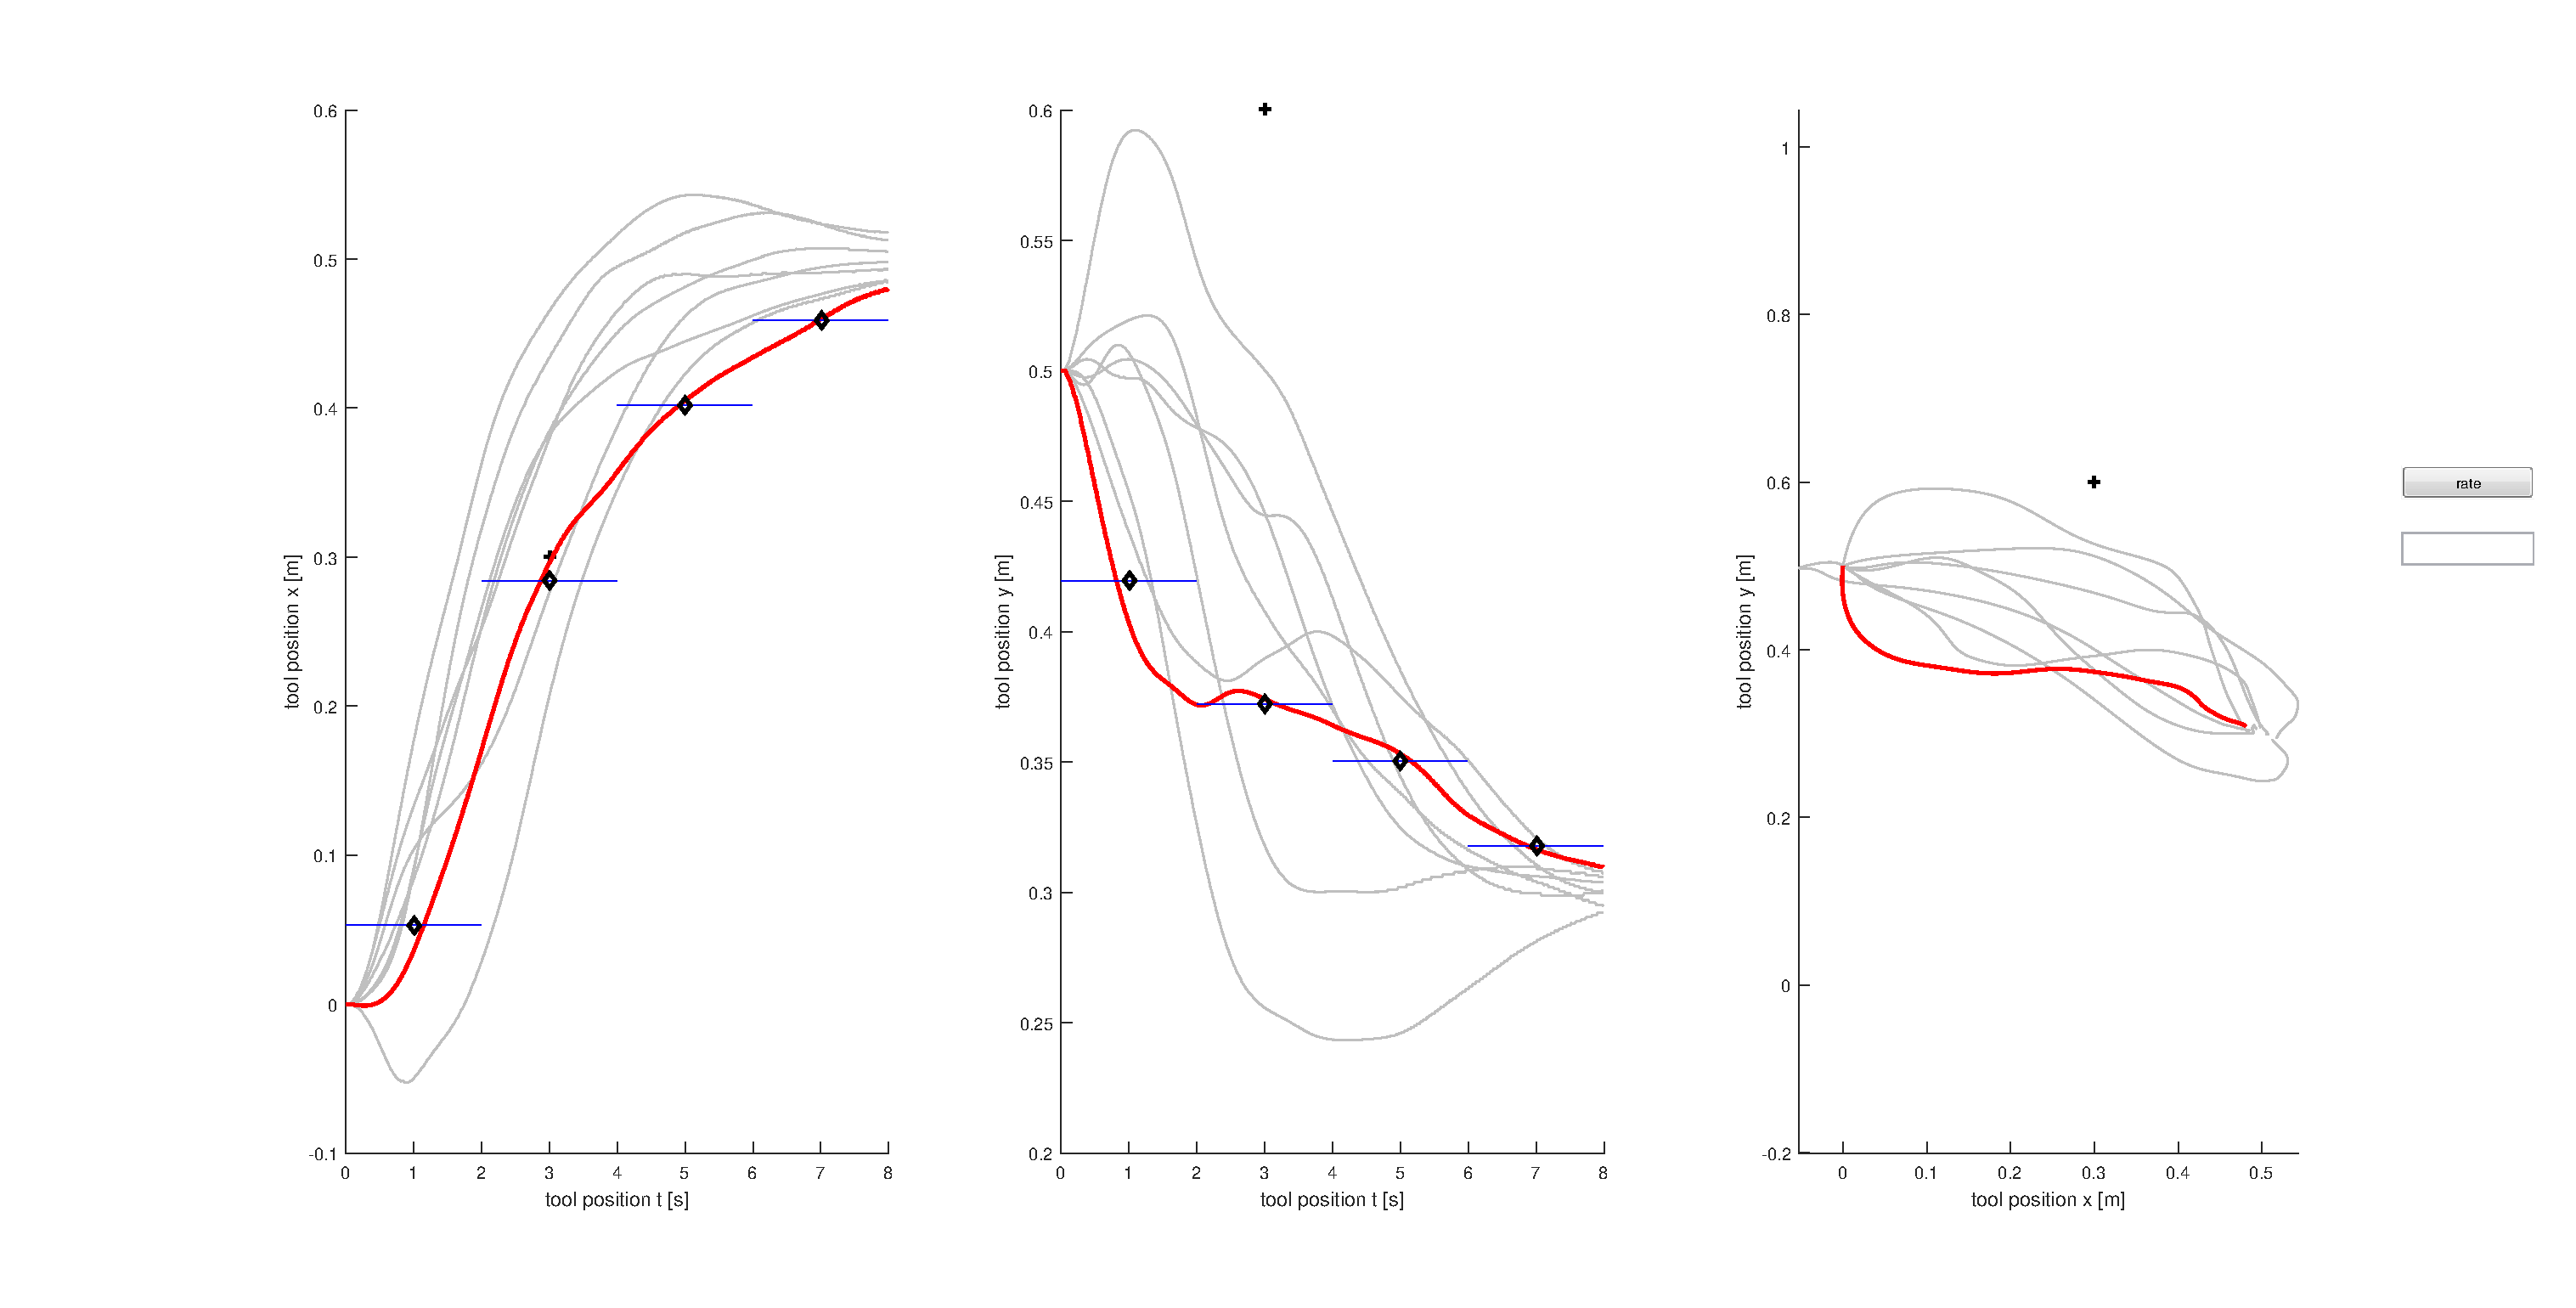
\includegraphics[width=0.7\textwidth, keepaspectratio=1]{figures/gui-single}
    \caption{Rating window used to rate demonstrations of full trajectories.}
    \label{fig:gui-expert-single}
\end{figure}%%
    
\begin{figure}[!htb]
    \centering
    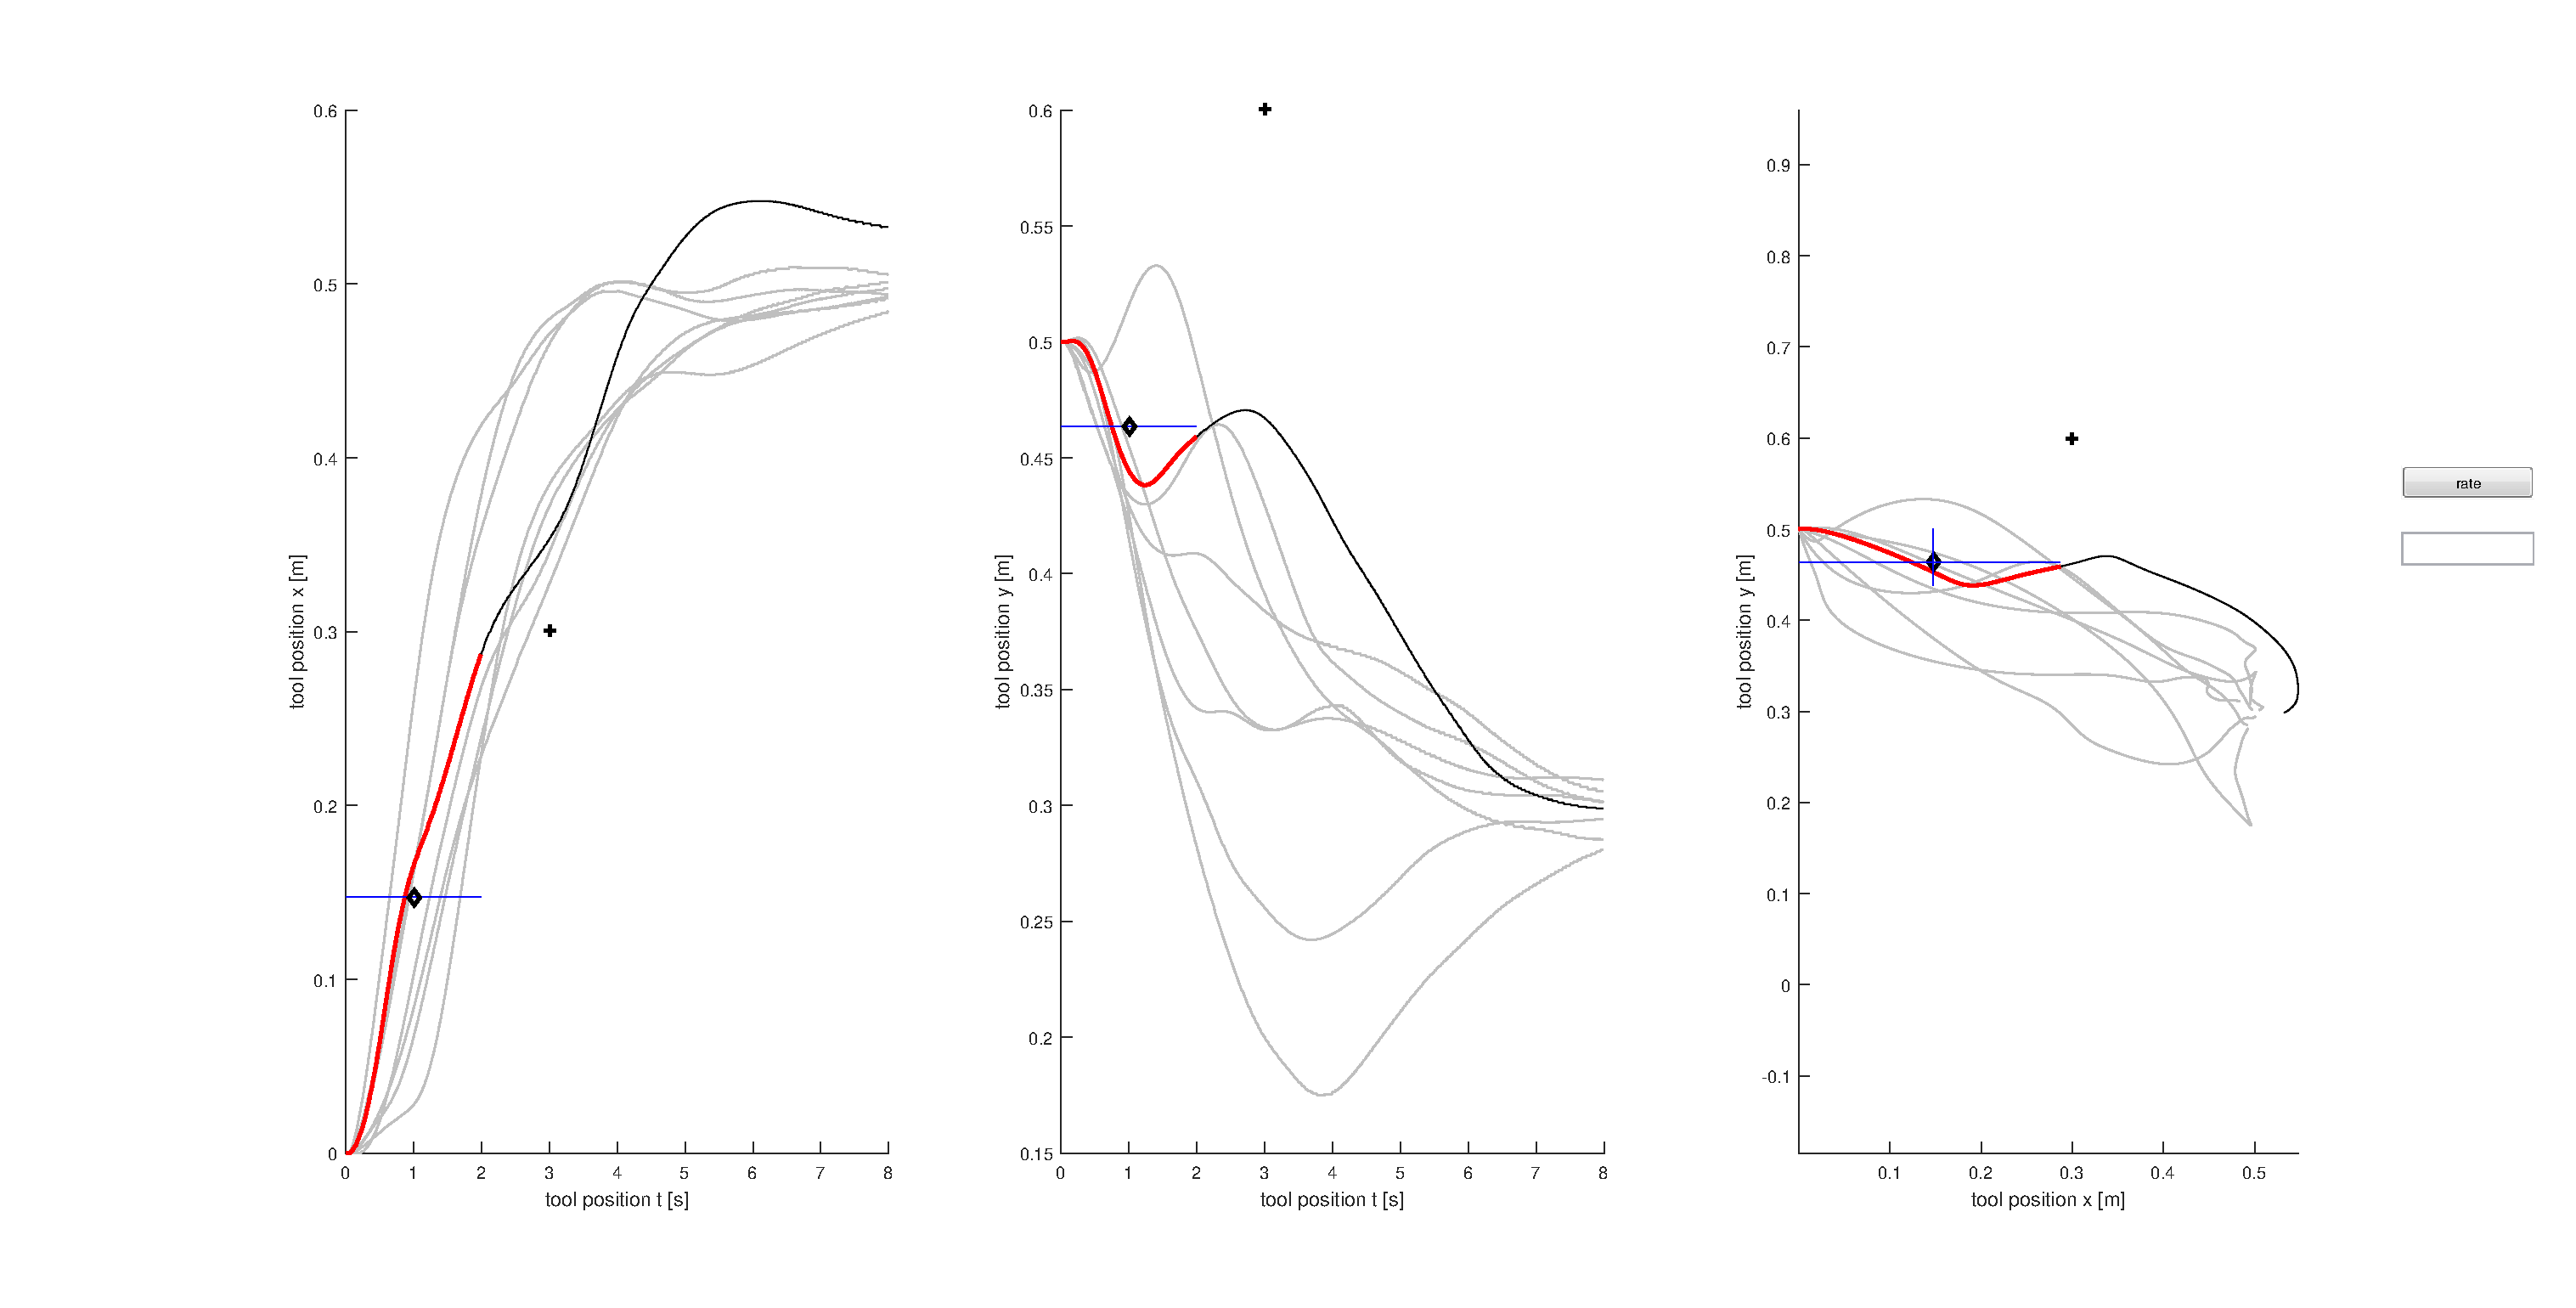
\includegraphics[width=0.7\textwidth, keepaspectratio=1]{figures/gui-multi}
    \caption{Rating window used to rate demonstrations of trajectory segments.}
    \label{fig:gui-expert-multi}
\end{figure}

\section{Single viapoint task}
\label{sec:vp}

In this section we will apply the two active reward learning algorithms we constructed to teach a robot arm a simple viapoint task. We will investigate if it is possible to teach a robot such a viapoint task purely based on expert feedback. As input for the reward model we will only use the average $x$ and $y$ position of the end effector, the variance of the end effector positions will not be used. First we will show the result of the algorithm using a computer expert. After that, the results of the algorithm with a human expert are shown. 

\subsection{Computer expert result}
The resulting trajectories of a viapoint task using a computer generated expert are on display in Figure \ref{fig:vp-single-noise-traject} and Figure \ref{fig:vp-multi-noise-traject}, where a single GP and a multi GP reward model is used respectively. In these figures, the average trajectory of twenty trials is shown as well as the standard deviation of the resulting trajectories. We also compare the results of the active reward learning algorithms with the results of a reinforcement learning algorithm, using the computer expert as a reward function. 

% Trajectory
\begin{figure}[!htb]
    \centering
    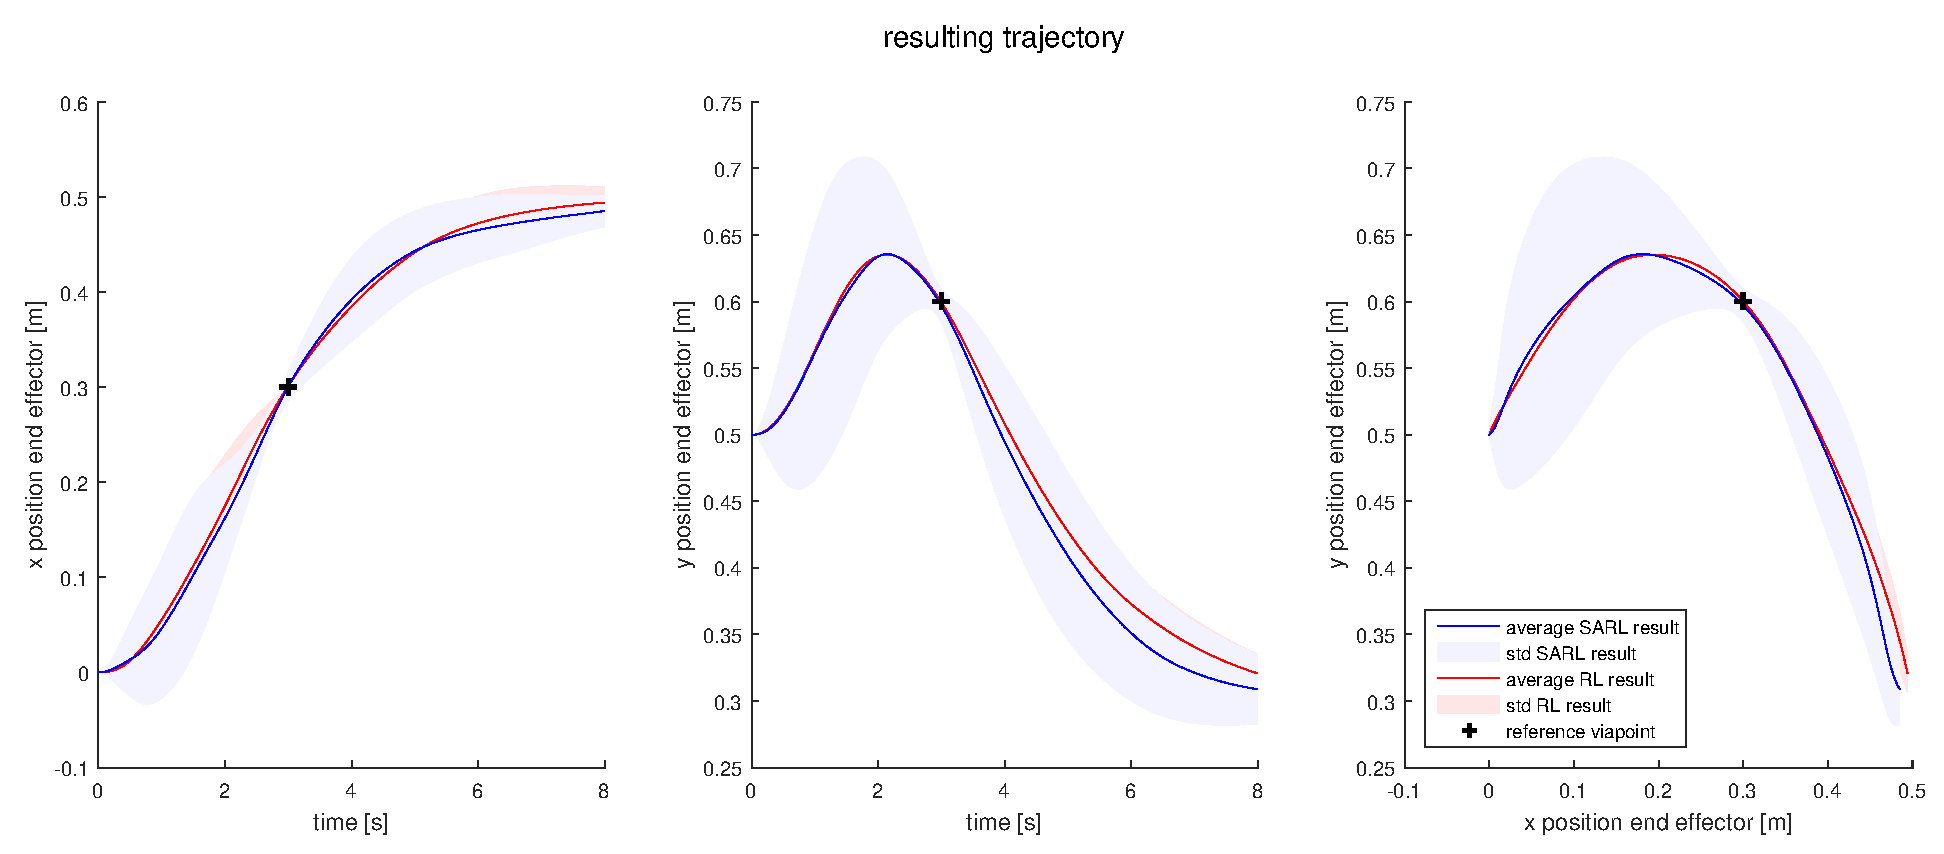
\includegraphics[width=\textwidth, height = 6 cm]{figures/results/viapoint/trajectory_single_noise_sum.eps}
    \caption{Resulting trajectory of a simple viapoint task using a single GP reward model.}
    \label{fig:vp-single-noise-traject}
\end{figure}

    
\begin{figure}[!htb]
    \centering
    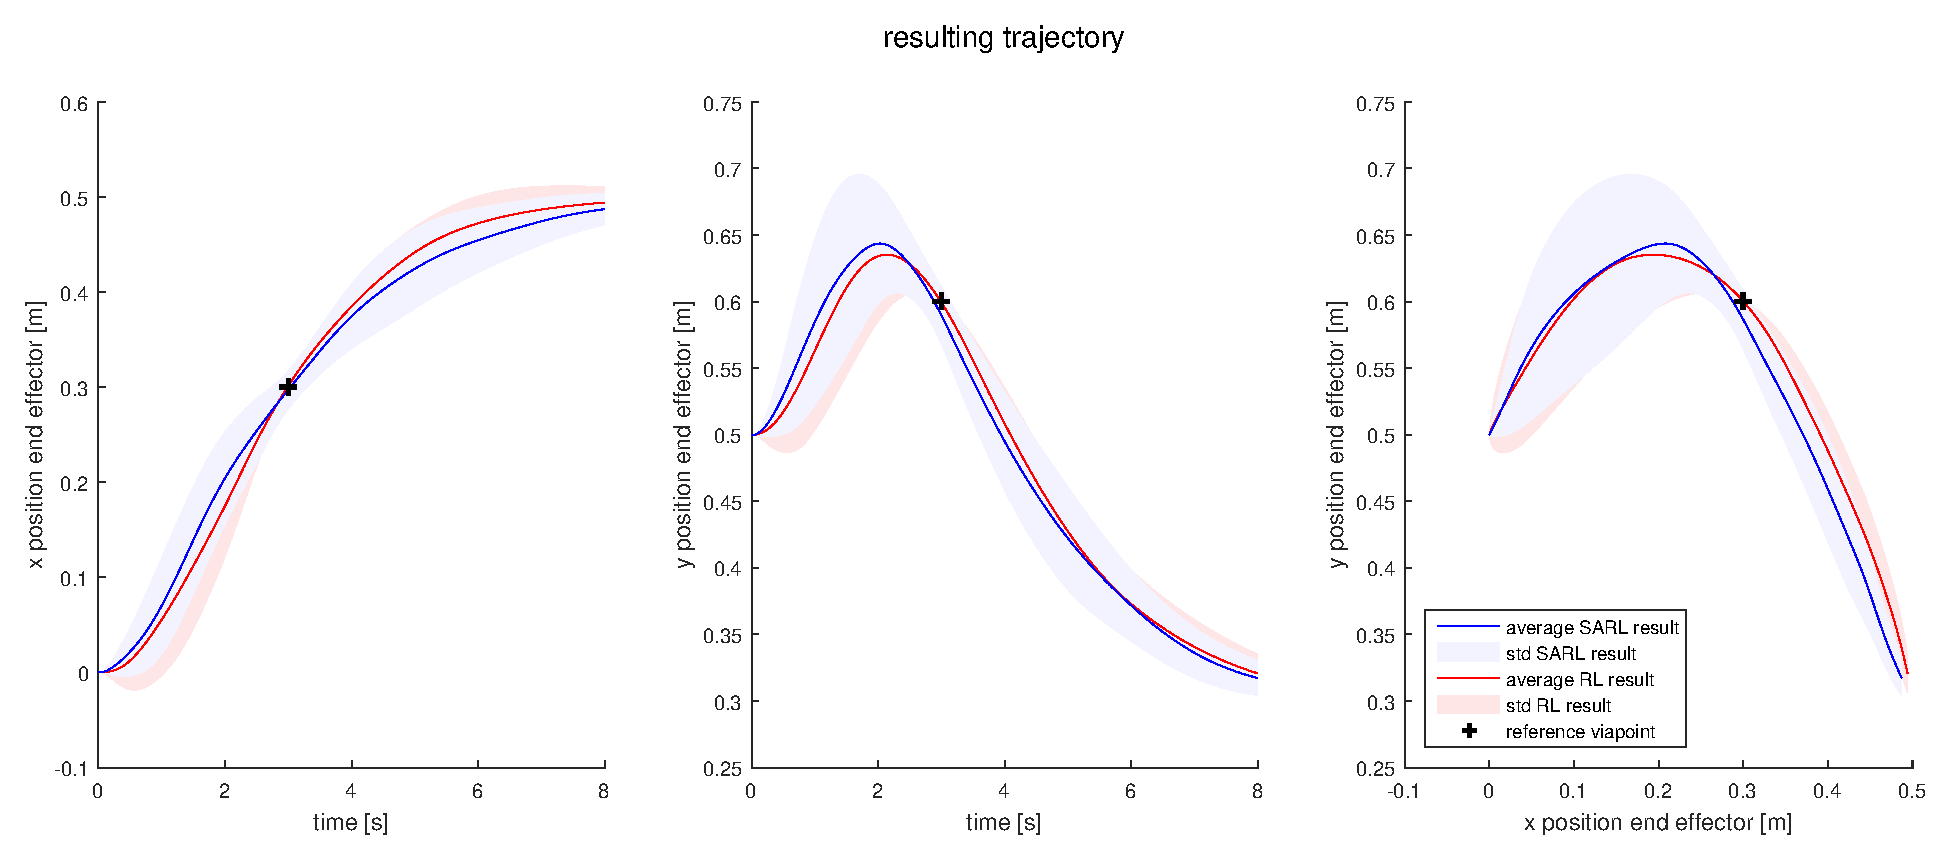
\includegraphics[width=\textwidth, height = 6 cm]{figures/results/viapoint/trajectory_multi_noise_sum.eps}
    \caption{Resulting trajectory of a simple viapoint task using a multi GP reward model.}
    \label{fig:vp-multi-noise-traject}
\end{figure}

It is clear from the resulting trajectories of the active reward learning method as well as the reinforcement learning algorithm that the preferred trajectory that crosses the viapoint is one in which the end effector approaches the viapoint from above. This is explained by the policy of the reinforcement learning agent. We use a dynamic movement primitive as a parametrization for our policy, which causes the trajectories to be drawn to a certain end goal point at the end of the trajectory. In case of our specific viapoint task, this end goal is placed below the viapoint. Since the reward model is only based on the average position of the end effector in a specific time segment, the agent will learn to approach the viapoint from above. 

Besides learning a decent policy that results in the end effector passing the viapoint, the reward function is also obtained in both algorithms. Since a computer expert is used, we can compare the obtained reward model with the ``true'' reward function. In the two figures below (Figure \ref{fig:vp-single-noise-con} and Figure \ref{fig:vp-multi-noise-con}), the reward learning process is visualized. It is clear from the figures that both single GP and the multi GP reward model are able to express the true reward with reasonable accuracy. However in both graphs it is clear that the difference between the reward model and the true reward does not converge to zero. Important to note here is that absolute difference between the reward model and the true reward function does not have to be a problem. The reinforcement learning method used in the experiments uses a softmax scaling method on the return of each trajectory in order to calculate the policy update (see Algorithm \ref{alg:PIBB}). This means that the reinforcement learning process is invariant under a scaling of the reward function. The only thing that matters is the relative difference in reward between different rollouts. 

\begin{figure}[!htb]
    \centering
    \begin{minipage}{.5\textwidth}
        \centering
        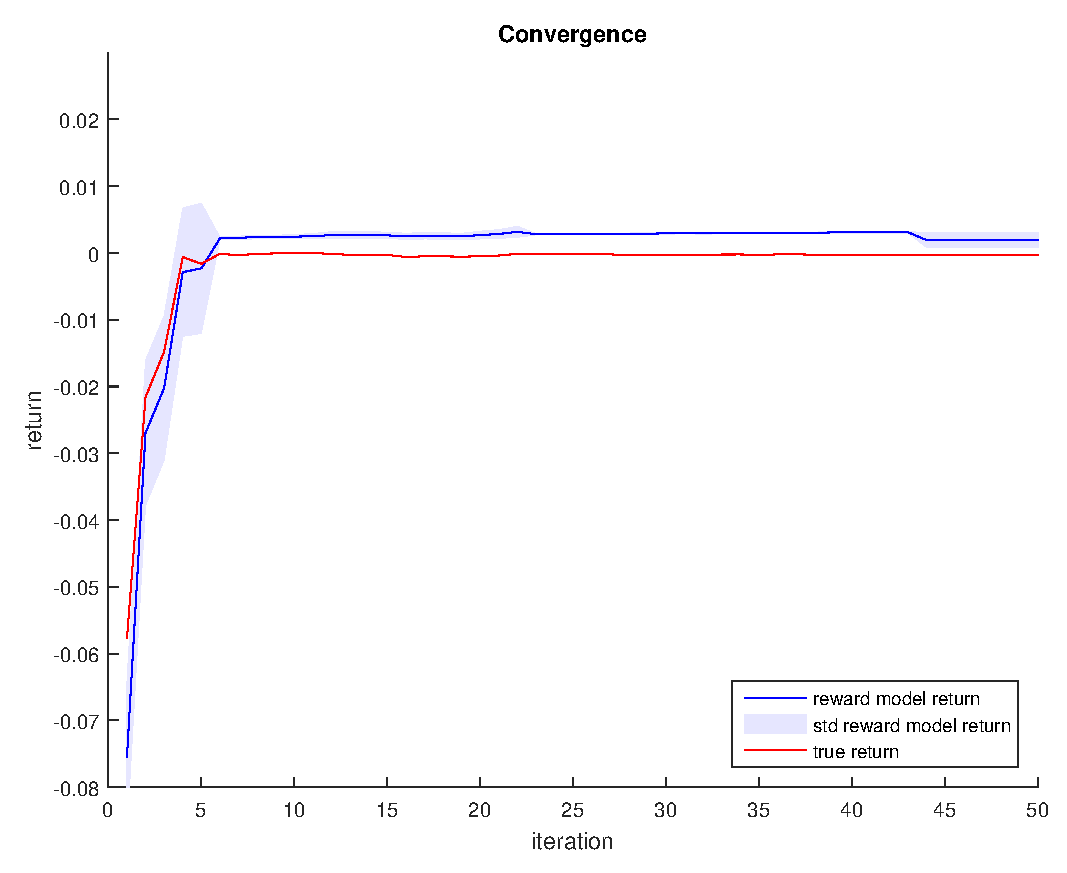
\includegraphics[width=\textwidth, keepaspectratio=1]{figures/results/viapoint/convergence_single_noise.eps}
        \caption{Convergence plot showing the return of the single GP reward model compared to the ``true'' return.}
        \label{fig:vp-single-noise-con}
    \end{minipage}%
    \begin{minipage}{0.5\textwidth}
        \centering
        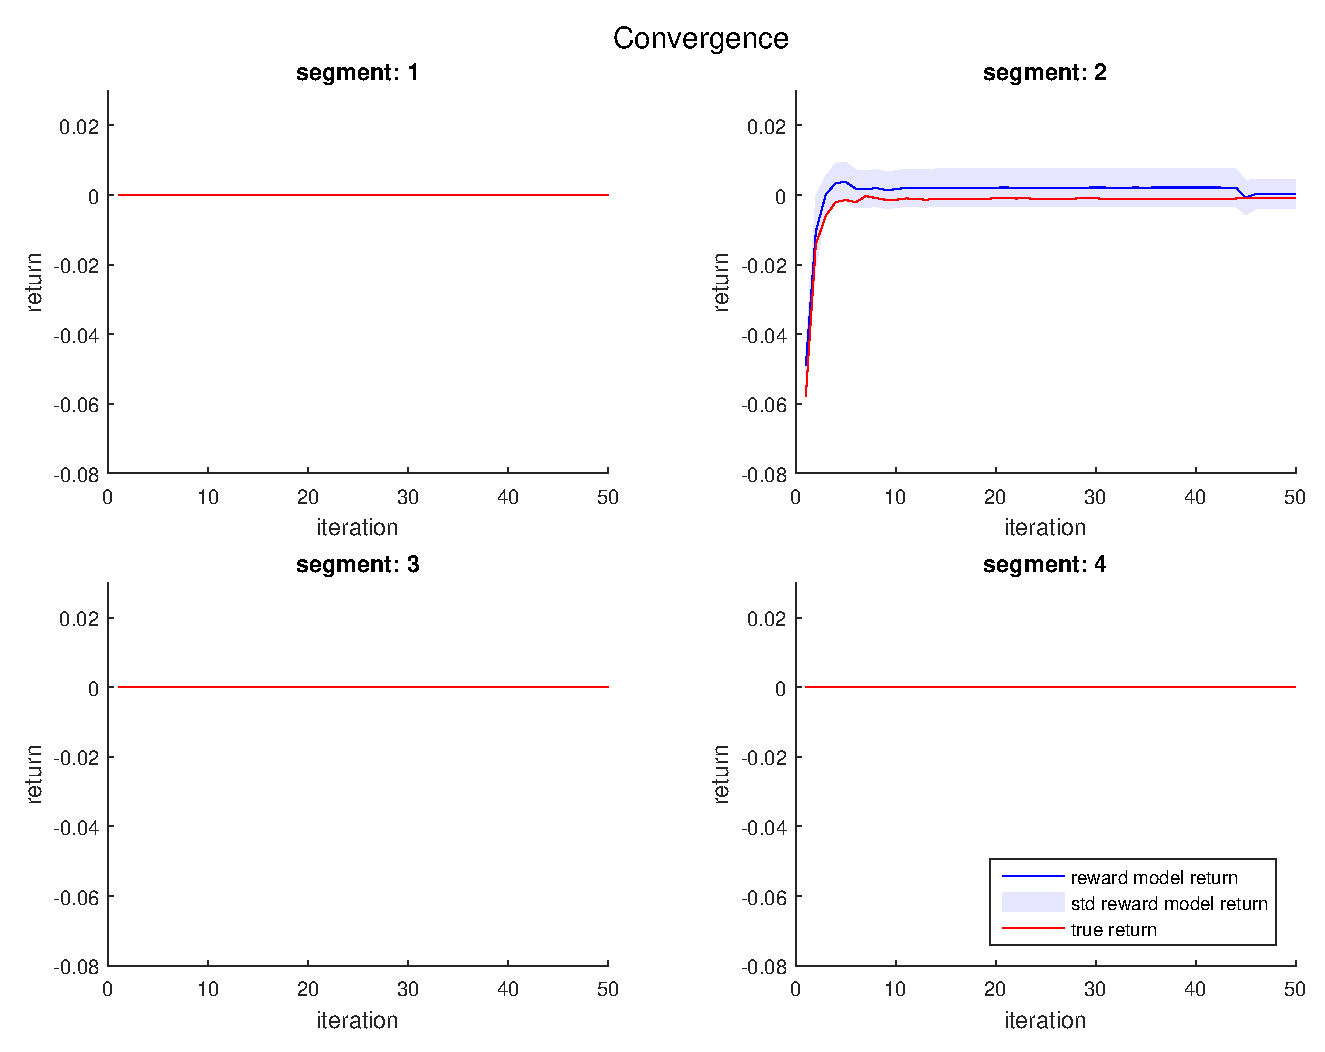
\includegraphics[width=\textwidth, keepaspectratio=1]{figures/results/viapoint/convergence_multi_noise.eps}
        \caption{Convergence plot showing the return of the multi GP reward model compared to the ``true'' return.}
        \label{fig:vp-multi-noise-con}
    \end{minipage}
\end{figure}

If we use a multi GP reward model, the only feature functions are used as input for each GP are the average $x$ and $y$ position of the end effector. This means that we are able to visualize the reward model, as can be seen in Figure \ref{fig:vp-multi-noise-reward}. The reward function of the first, third and last segment are all zero functions, since no tasks are placed in these time segments. In the second time segment we can clearly observe an optimum, which collides with the viapoint. Important to note is that an initial number of eight rollouts are used for initializing the reward model. During learning, the only extra demonstrations are performed in the second segment of the trajectory.
% results multi gp

% Reward function
\begin{figure}[!htb]
\centering
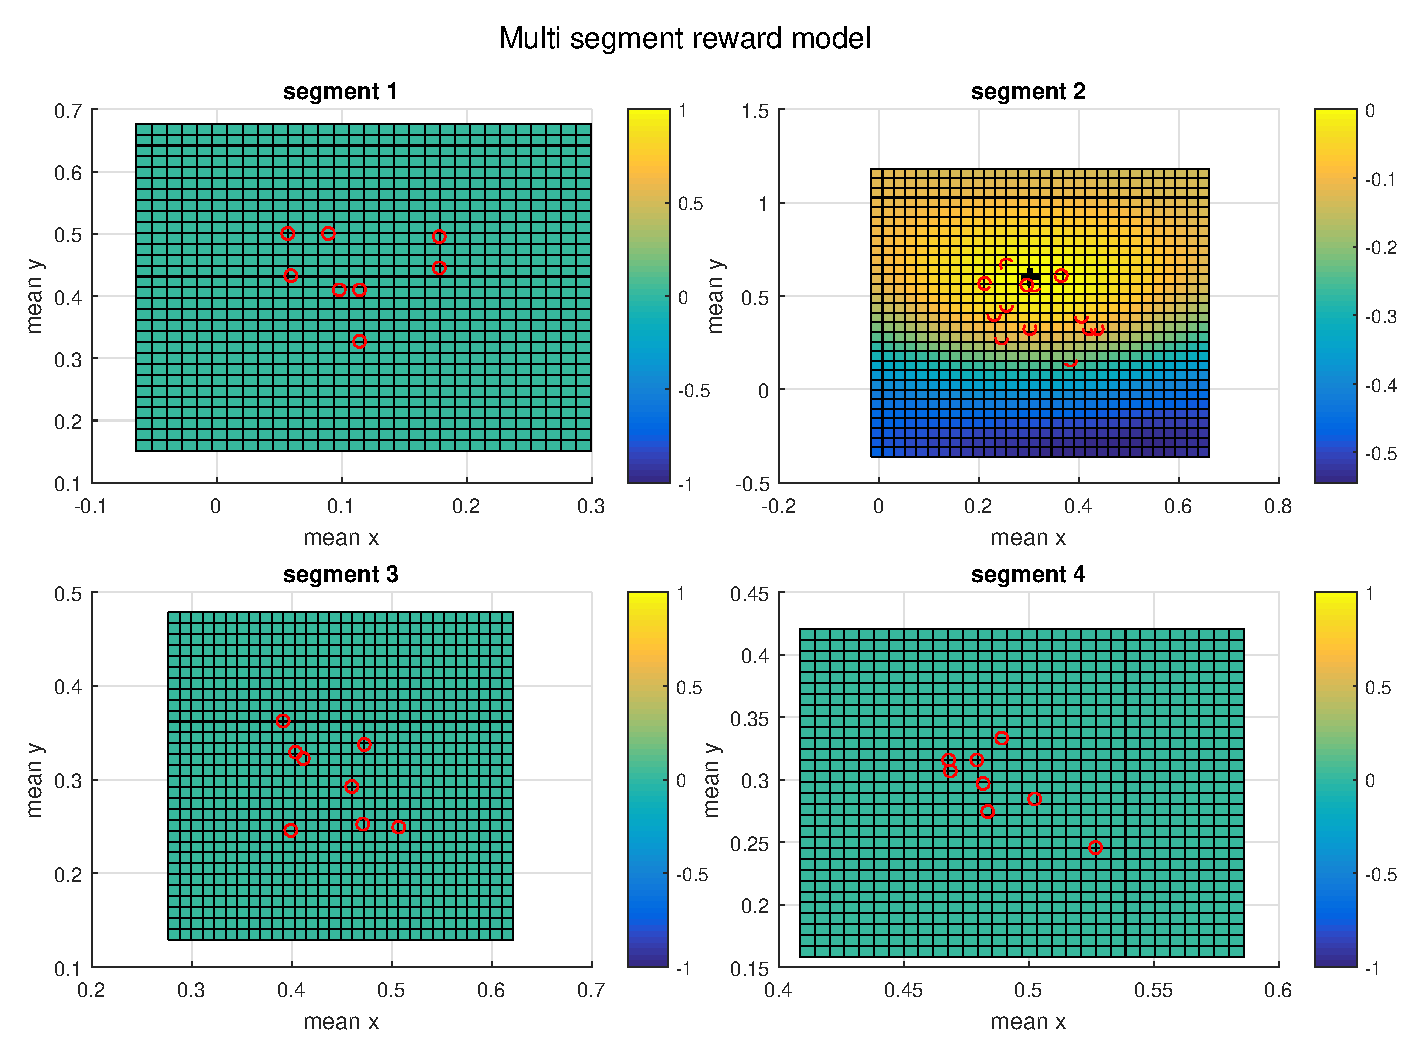
\includegraphics[width=\textwidth, keepaspectratio=1]{figures/results/viapoint/return_flat_multi_noise.eps}
\caption{Graphical representation of the resulting reward function of a multi GP reward model. The red dots represent queried rollouts. The black mark denotes the viapoint.}
\label{fig:vp-multi-noise-reward}
\end{figure}

Now that the qualitative properties of the results are discussed we can focus on the quantitative measures of the algorithms. In this task there are two distinct measures we can use to judge the performance on. Foremost, we use the distance of the end effector to the viapoint $\bm{x}_{\text{viapoint}}$ at time $t_{\text{viapoint}}$. Secondly, we would like to keep the amount of expert queries to a minimum. In Table \ref{tab:vp-com}, the resulting measures of twenty attempts are summarized for each algorithm. We compare the SARL algorithms with a  $\text{PI}^{BB}$ RL method that uses the computer expert as its reward function. 

It is clear that for this simple viapoint task, the single GP algorithm is a better choice in terms of performance. First off, the average distance to the viapoint is lower compared to the multi GP method. Also, the total amount of expert queries is significantly lower. Important to note is that the multi GP method needs more expert queries to initialize its reward model, since each of the individual segments needs to be initialized with segment specific ratings. The number of queries needed during learning is actually lower when using a multi GP reward model. If we compare the SARL algorithms results with the results of $\text{PI}^{BB}$ we can conclude that using a programmed reward function is still a significantly better choice for this simple task.

\begin{table}[!htb]
    \centering
    \caption{Results of segmented active reward learning and $\text{PI}^{BB}$ applied to a viapoint task using a computer expert.}
    \label{tab:vp-com}
    \begin{tabular}{|p{6cm}|c|c|c|c|}
        \hline
        Measure & single GP & multi GP & $\text{PI}^{BB}$ RL & Unit \\ \hline \hline
        Average distance viapoint & $1.5 \cdot 10^{-2}$ & $2.3 \cdot 10^{-2}$ & $7.5 \cdot 10^{-4}$ & \si{m}  \\ \hline
        Standard deviation distance viapoint & $2.08 \cdot 10^{-2}$ & $1.21 \cdot 10^{-2}$ & $4.9 \cdot 10^{-4}$ & \si{m} \\ \hline
        Initial number expert queries & 8 & 32 & 0 & - \\ \hline
        Average number expert queries & 20.5 & 40.35 & 0 &  - \\ \hline
        Standard deviation number expert queries & 3.8 & 3.5 & 0 &  - \\ \hline 
    \end{tabular}
\end{table}

\clearpage

\subsection{Manual expert result}
Now that we have shown the results of segmented active reward learning using a computer expert, we will show the results the same two algorithms using a human expert (the author). The computer rated algorithm is not completely identical to the human rated algorithm. Besides the fact that the input for demonstrations ratings is different, the tolerance parameter for expected policy divergence is also increased. This is due to a higher rating noise that the human expert is expected to produce. Keeping this tolerance parameter unchanged would blow up the number of demonstrations. 

The resulting trajectories are on display in Figure \ref{fig:vp-single-manual-traject} and Figure \ref{fig:vp-multi-manual-traject}. It can easily be observed that the viapoints are not tracked as well with the human expert rating the trajectories compared to the computer expert. 

% Trajectory
\begin{figure}[!htb]
    \begin{minipage}[b]{\linewidth}
        \centering
        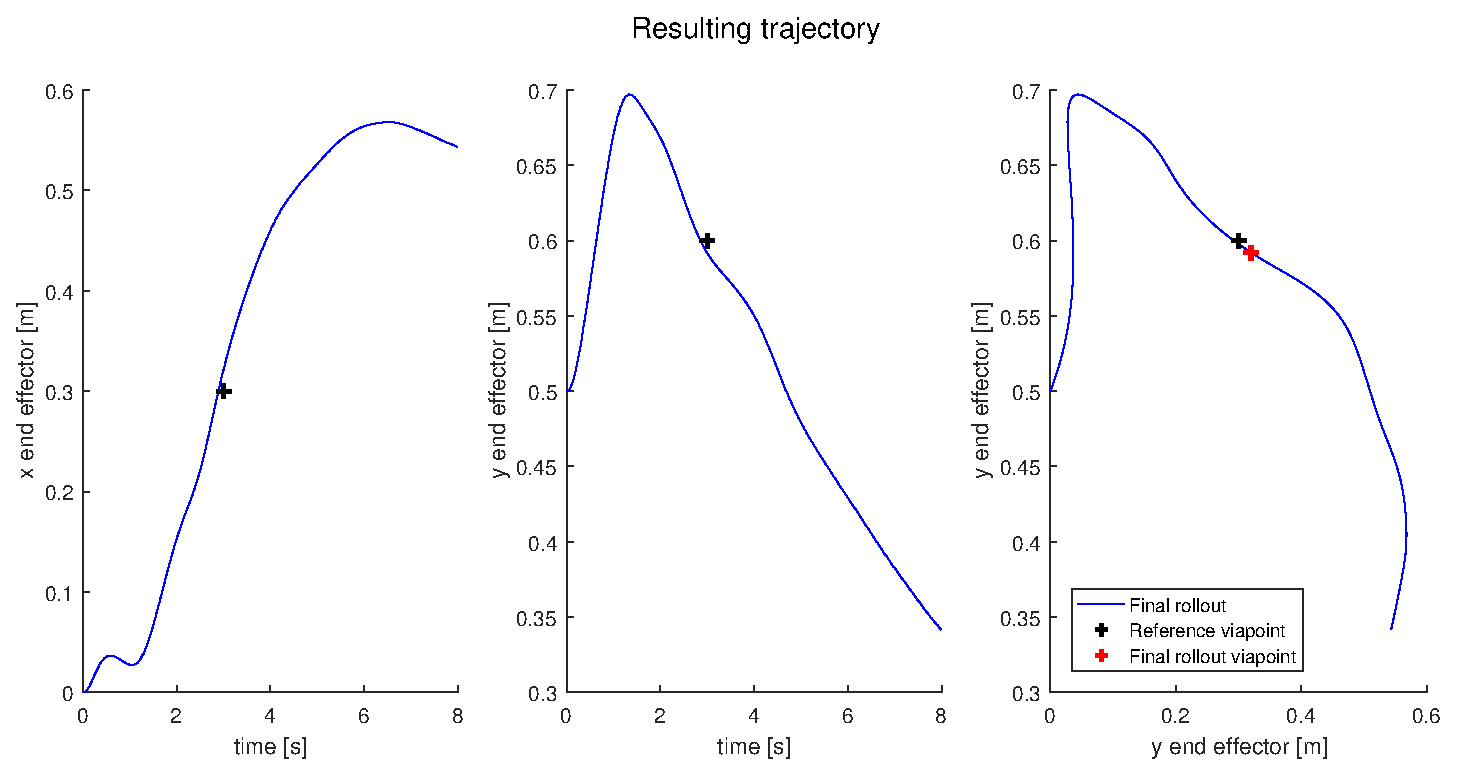
\includegraphics[width=\textwidth, height = 6cm]{figures/results/viapoint/trajectory_single_manual.eps}
        \caption{Resulting trajectory of a simple via point task using a single GP reward model.}
        \label{fig:vp-single-manual-traject}
        \vspace{4ex}
    \end{minipage}%%
    
    \begin{minipage}[b]{\linewidth}
        \centering
        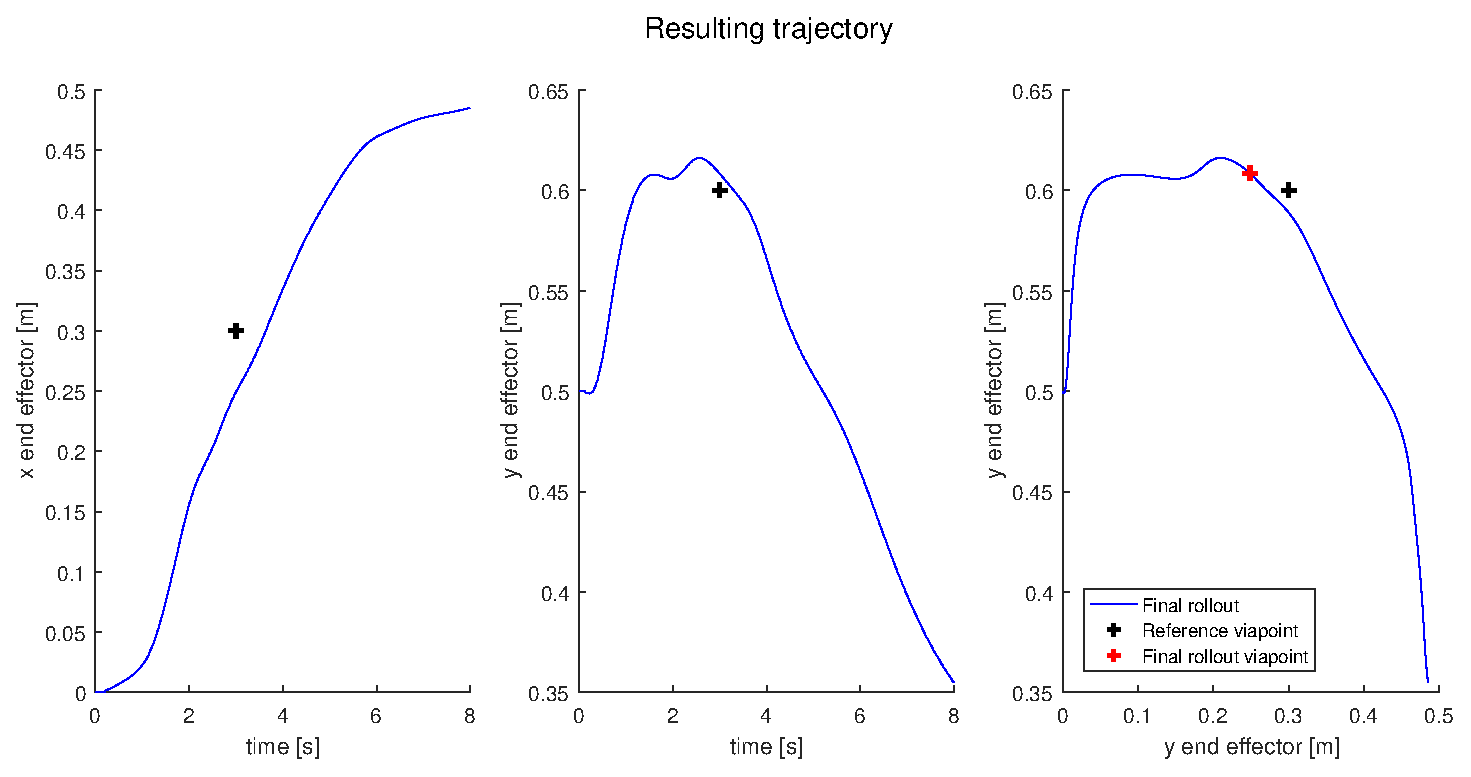
\includegraphics[width=\textwidth, height = 6cm]{figures/results/viapoint/trajectory_multi_manual.eps}
        \caption{Resulting trajectory of a simple via point task using a multi GP reward model.}
        \label{fig:vp-multi-manual-traject}
    \end{minipage}%%
\end{figure}

The resulting trajectories show a preference for approaching the viapoint from above as was observed in the previous section. It is difficult to create a reward function that prefers more elegant solutions, such as an approach from below, since the inputs for the reward model only contain information about the average position of the end effector. The expert cannot alleviate this problem.

Since we do not have a ``true'' reward function at our disposal, we cannot use this for comparing the reward learning process. Instead we will compare the convergence of the reward model with the ratings that are given by the human expert, as is visible in Figure \ref{fig:vp-single-manual-con} and Figure \ref{fig:vp-multi-manual-con}. 

A few observations can be made from these convergence plots. First off, the single GP reward model requires more expert queries than the multi GP reward model. This was not observed in the computer rated algorithm in the previous section. The reason for this amount of queries can be found in the rating noise, which is a lot higher using a human expert. 

A typical aspect of the human rated algorithm is that the expert is allowed to choose his or her own rating scale. So the fact that the single GP reward model shows a higher expert return in the later stages compared to the multi GP reward model does not mean anything, as we observed in the trajectory plots that the resulting trajectory of the multi GP model is actually better. The only task of the human expert is to teach the robot which rollouts are better or worse, relative to what has been rated before. Using a Gaussian process as a reward model in combination with the $\text{PI}^{BB}$ reinforcement learning algorithm allows the human expert to use whatever rating scale he or she prefers.  


\begin{figure}[!htb]
    \centering
    \begin{minipage}{.5\textwidth}
        \centering
        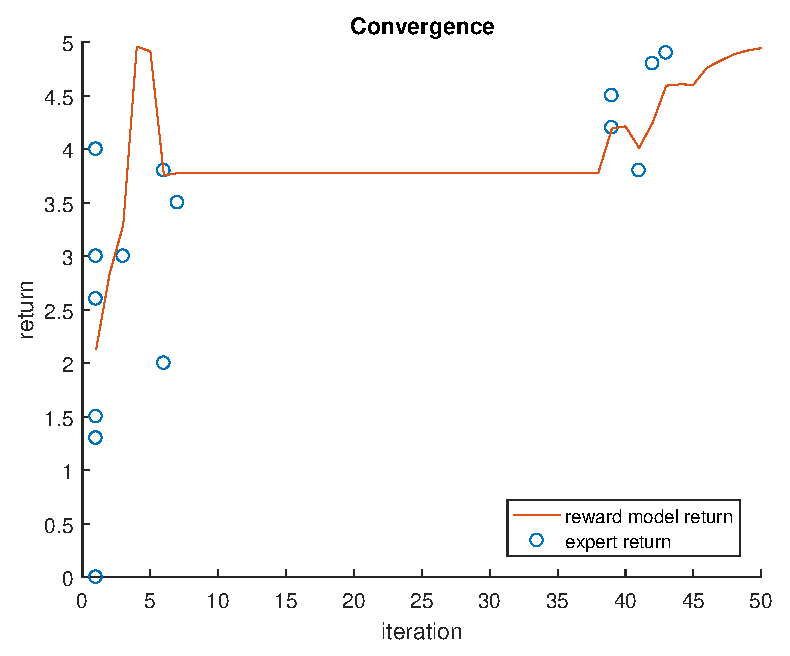
\includegraphics[width=\textwidth, keepaspectratio=1]{figures/results/viapoint/convergence_single_manual.eps}
        \caption{Convergence plot showing the return of the single GP reward model compared to the expert return.}
        \label{fig:vp-single-manual-con}
    \end{minipage}%
    \begin{minipage}{0.5\textwidth}
        \centering
        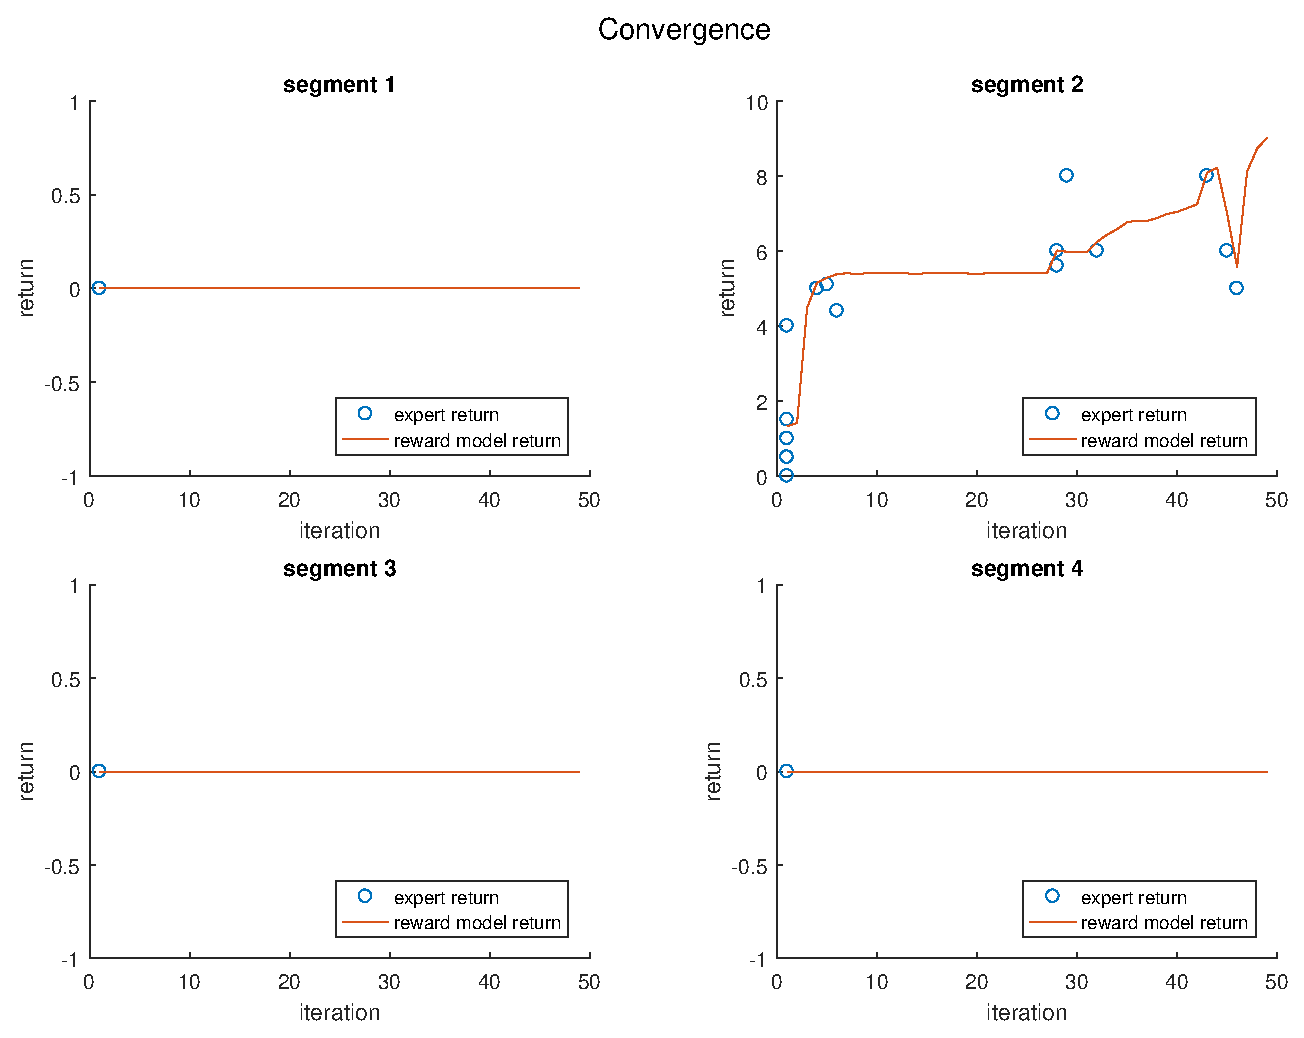
\includegraphics[width=\textwidth, keepaspectratio=1]{figures/results/viapoint/convergence_multi_manual.eps}
        \caption{Convergence plot showing the return of the multi GP reward model compared to the expert return.}
        \label{fig:vp-multi-manual-con}
    \end{minipage}
\end{figure}

The reward function of the multi GP reward model can be visualized as well. In Figure \ref{fig:vp-multi-manual-reward} the reward functions of the different time segments are on display. As expected, the GPs of the non-relevant segments all return zero. We can also see that the reward function of the second segment shows a clear optimum at the viapoint position, but the gradient around this optimum is much higher than observed with the computer rated algorithm. This applies even you ignore the fact that the scaling of the expert ratings is different.


% Reward function
\begin{figure}[!htb]
\centering
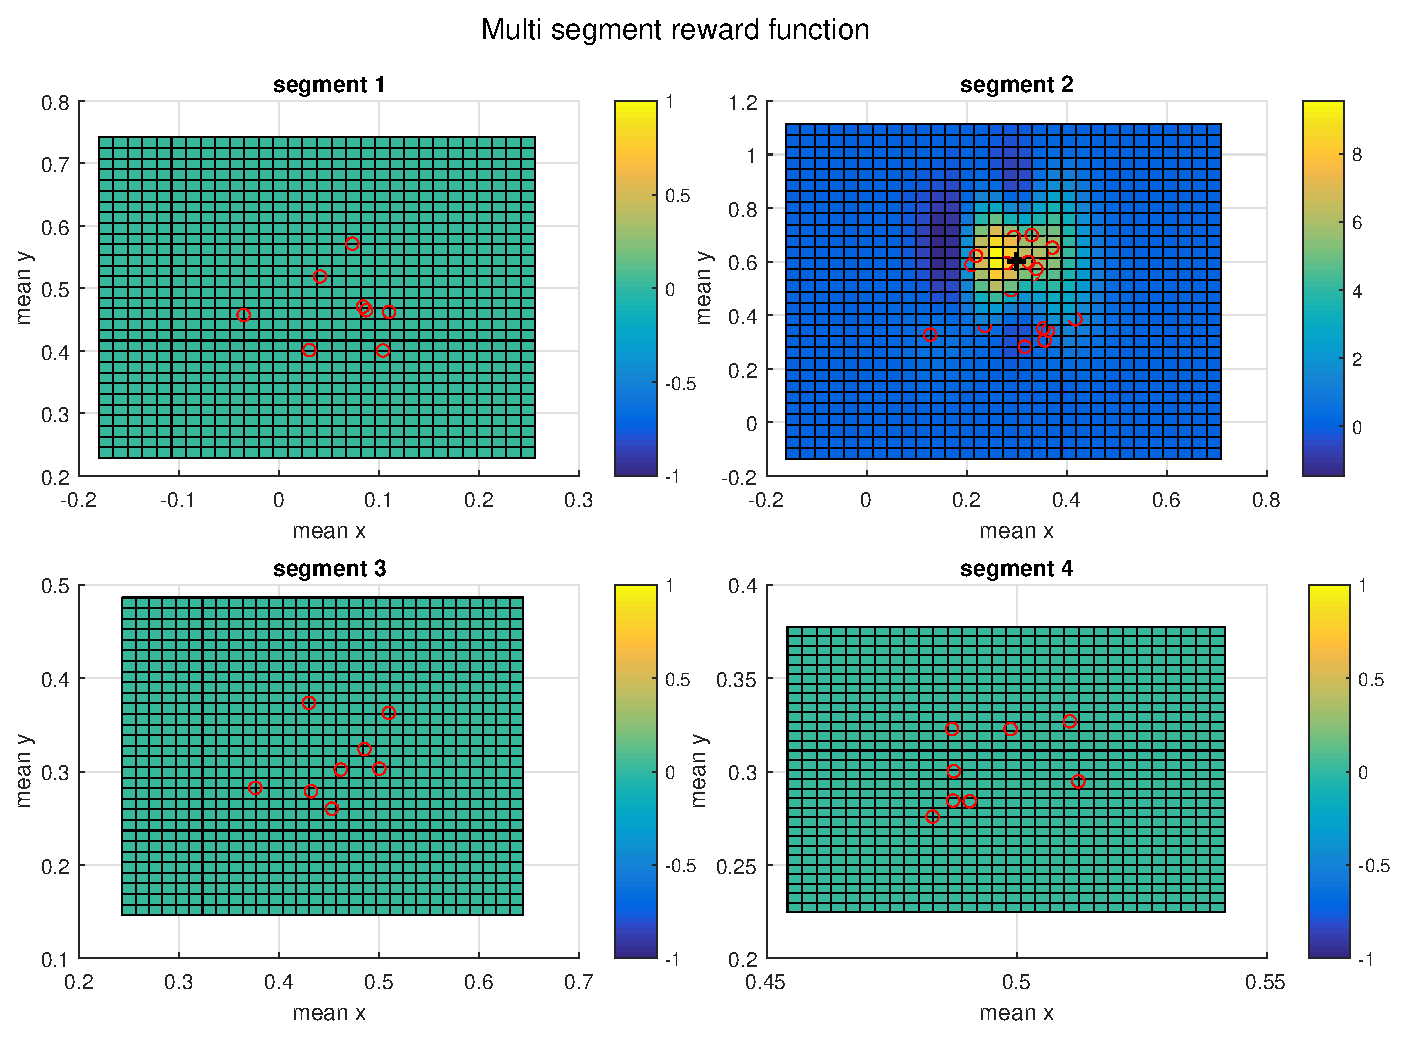
\includegraphics[width=\textwidth, keepaspectratio=1]{figures/results/viapoint/return_flat_multi_manual.eps}
\caption{Graphical representation of the resulting reward function of a multi GP reward model. The red dots represent queried rollouts. The black mark denotes the viapoint.}
\label{fig:vp-multi-manual-reward}
\end{figure}

In Table \ref{tab:vp-com-man} the results of the two manual trials are compared with the $\text{PI}^{BB}$ RL method. It is clear from the table that the $\text{PI}^{BB}$ method still outperforms both reward learning methods, since the $\text{PI}^{BB}$ viapoint tracking measure is two orders of magnitude both reward learning methods. 

If we compare the results of the manual trials in Table \ref{tab:vp-com-man} with the results of the computer expert in Table \ref{tab:vp-com-man}, we see that the viapoint tracking performance of the computer generated results is clearly better. It is also clear that when a human expert is used, the number of expert queries is significantly higher than when we use a computer expert. This difference clearly suggests that the rating noise variance used in the computer expert was lower than the human experts rating noise.

From the results table, it is also easy to note that the single GP reward model is a better choice for this task compared to the multi GP reward model. In terms of expert queries, the single GP variant also performs better, even if we neglect the initial demonstrations and the viapoint tracking performance is over twice as good.

\begin{table}[!htb]
    \centering
    \caption{Results of segmented active reward learning and $\text{PI}^{BB}$ applied to a viapoint task using a human expert.}
    \label{tab:vp-com-man}
    \begin{tabular}{|p{6cm}|c|c|c|c|}
        \hline
        Measure & single GP & multi GP & $\text{PI}^{BB}$ RL & Unit \\ \hline \hline
        Distance viapoint & $2.14 \cdot 10^{-2}$ & $5.2 \cdot 10^{-2}$ & $7.5 \cdot 10^{-4}$ & \si{m}  \\ \hline
        Initial number expert queries & 8 & 32 & 0 & - \\ \hline
        Number expert queries & 17 & 43 & 0 &  - \\ \hline
    \end{tabular}
\end{table}


\section{Multi objective task}
\label{sec:ad}

In Section \ref{sec:vp} we described how we can teach a viapoint task to a robotic arm. We will investigate the performance for teaching the robot a more difficult task in this section. This task will contain two objectives. First off, we will recycle the viapoint objective that we used in Section \ref{sec:vp}. Besides that, the end effector of the robot arm must track a flat plane in space at the end of the trajectory. This second objective is harder to achieve for the robot arm. Also the combination of two objectives makes this task more challenging to solve.

\subsection{Computer expert result}
\label{sec:com-ad}
The computer expert described in Section \ref{sec:vp} needs to be extended in order to be used for the new task description. We add a term which penalizes deviation from the viaplane in the last time segment. Also we need to multiply the result of the individual objectives (viapoint and viaplane) with a weight parameter, such that the importance of the two objectives is scaled properly. 

In Figure \ref{fig:adx-single-noise-traject} the average resulting trajectories of multiple succeeded runs using the single GP model is on display. A plot showing the resulting trajectories of the algorithm using a multi GP reward model is shown in Figure \ref{fig:adx-multi-noise-traject}. Both trajectories clearly show an attraction towards the viapoint and the viaplane. We can already observe that the single GP reward model does not track the viapoint as accurate as is the case with a single objective task. In the trajectory plot of the single GP reward model we see that the standard deviation around the viapoint is significantly higher. Apparently, the single GP reward model does not map the multi objective reward function as well as the multi GP reward model. 

% Trajectory
\begin{figure}[!htb]
    \begin{minipage}[b]{\linewidth}
        \centering
        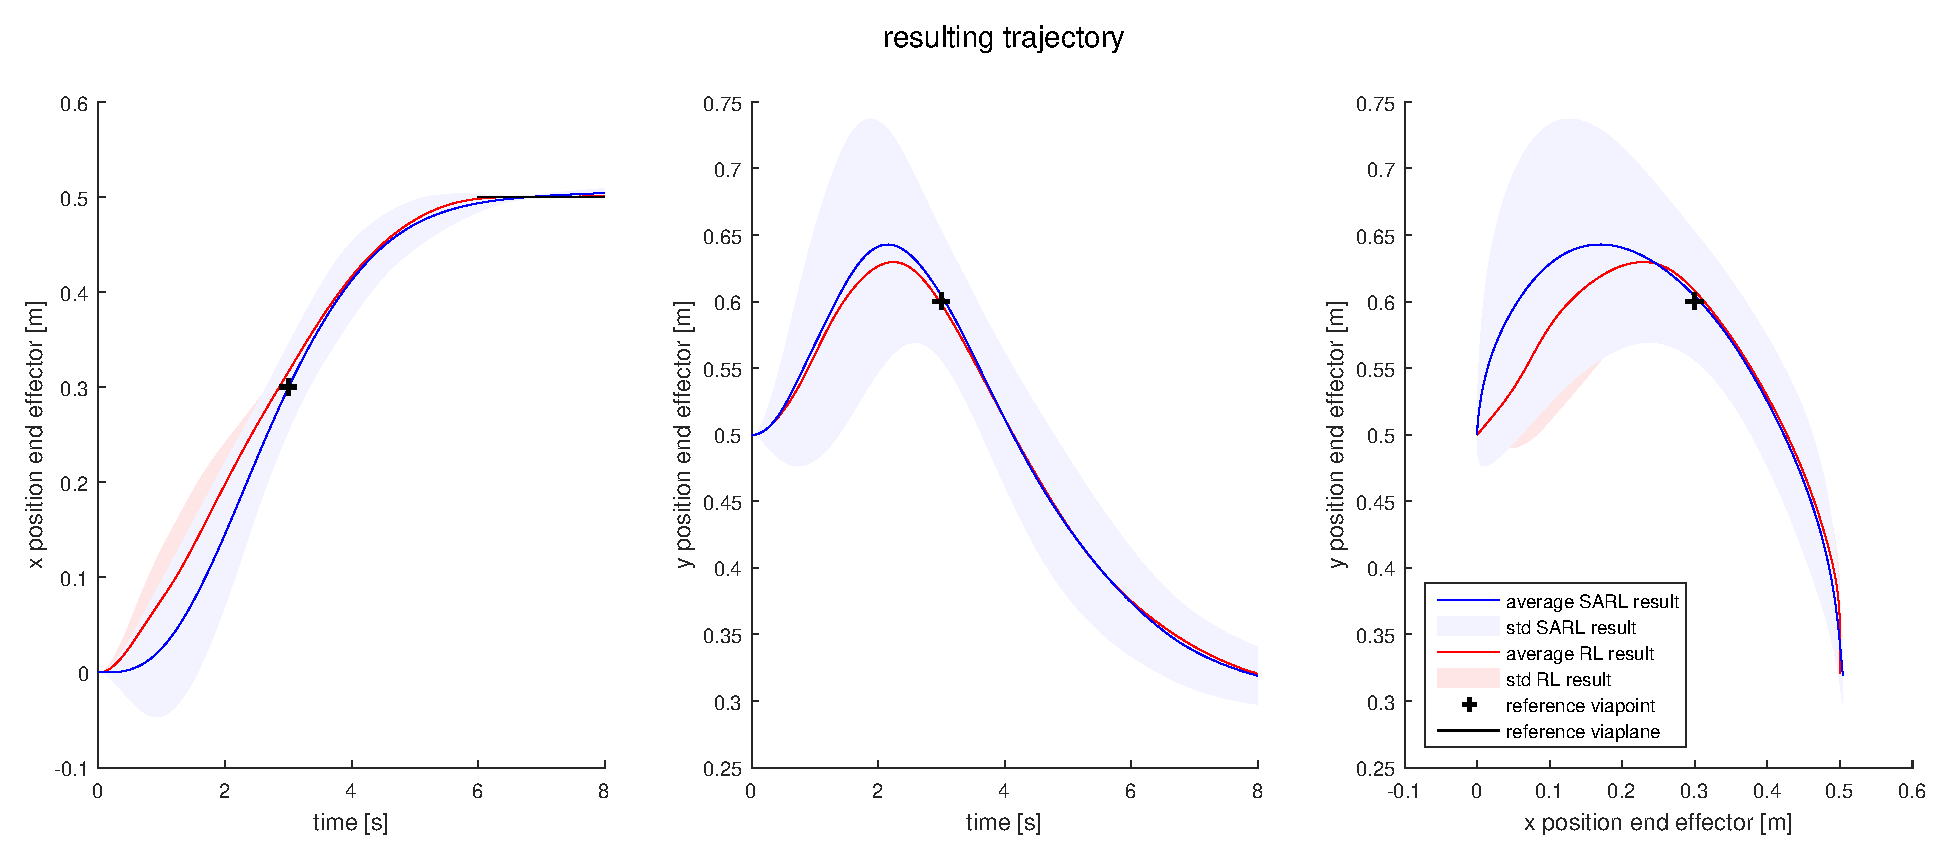
\includegraphics[width=\textwidth, height = 6 cm]{figures/results/advancedx/trajectory_single_noise_sum.eps}
        \caption{Resulting trajectory of a multi objective task using a single GP reward model.}
        \label{fig:adx-single-noise-traject}
        \vspace{4ex}
    \end{minipage}%%
    
    \begin{minipage}[b]{\linewidth}
        \centering
        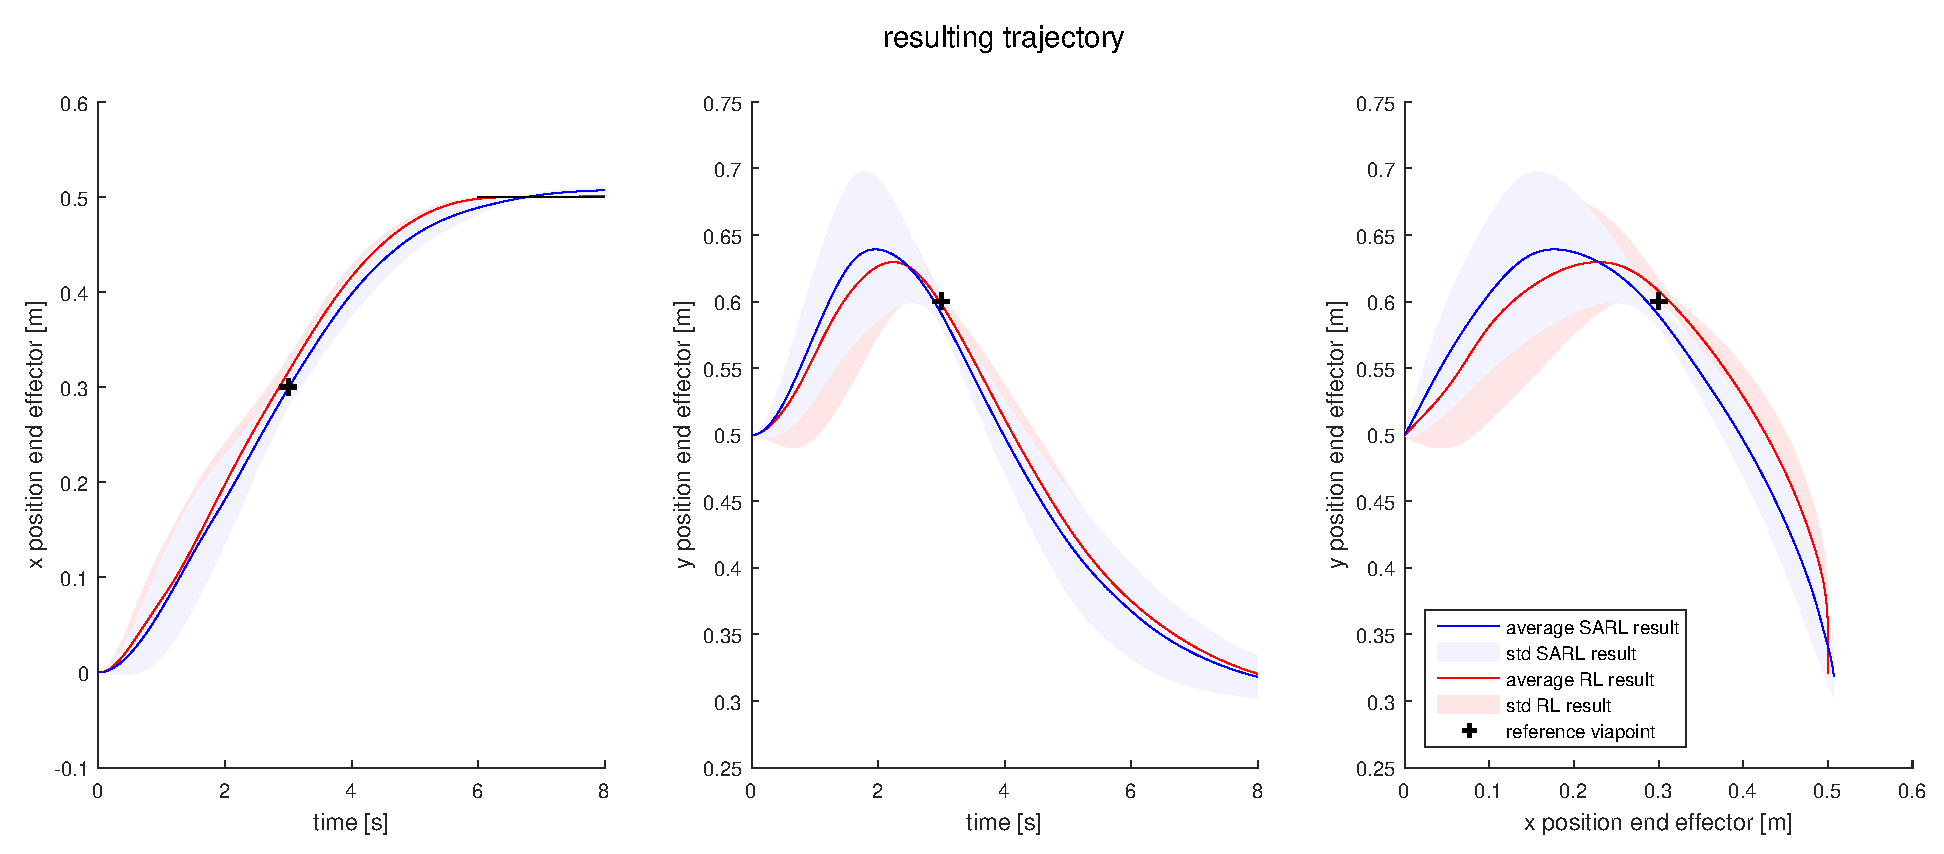
\includegraphics[width=\textwidth, height = 6 cm]{figures/results/advancedx/trajectory_multi_noise_sum.eps}
        \caption{Resulting trajectory of a multi objective task using a multi GP reward model.}
        \label{fig:adx-multi-noise-traject}
    \end{minipage}%%
\end{figure}

If we look at the convergence plots (Figures \ref{fig:adx-single-noise-con} and \ref{fig:adx-multi-noise-con}) we can make some remarks regarding the stability issues. As can be seen in the convergence of a successful run using a single GP as reward model, it is clear that the reward model does not converge as fast as before. The reward model has a tendency to overestimate the return of trajectories and needs to be severely corrected during learning. If we look at the convergence plot of the multi GP reward model (Figure \ref{fig:adx-multi-noise-con}), we observe a much more stable learning algorithm.


\begin{figure}[!htb]
    \centering
    \begin{minipage}{.5\textwidth}
        \centering
        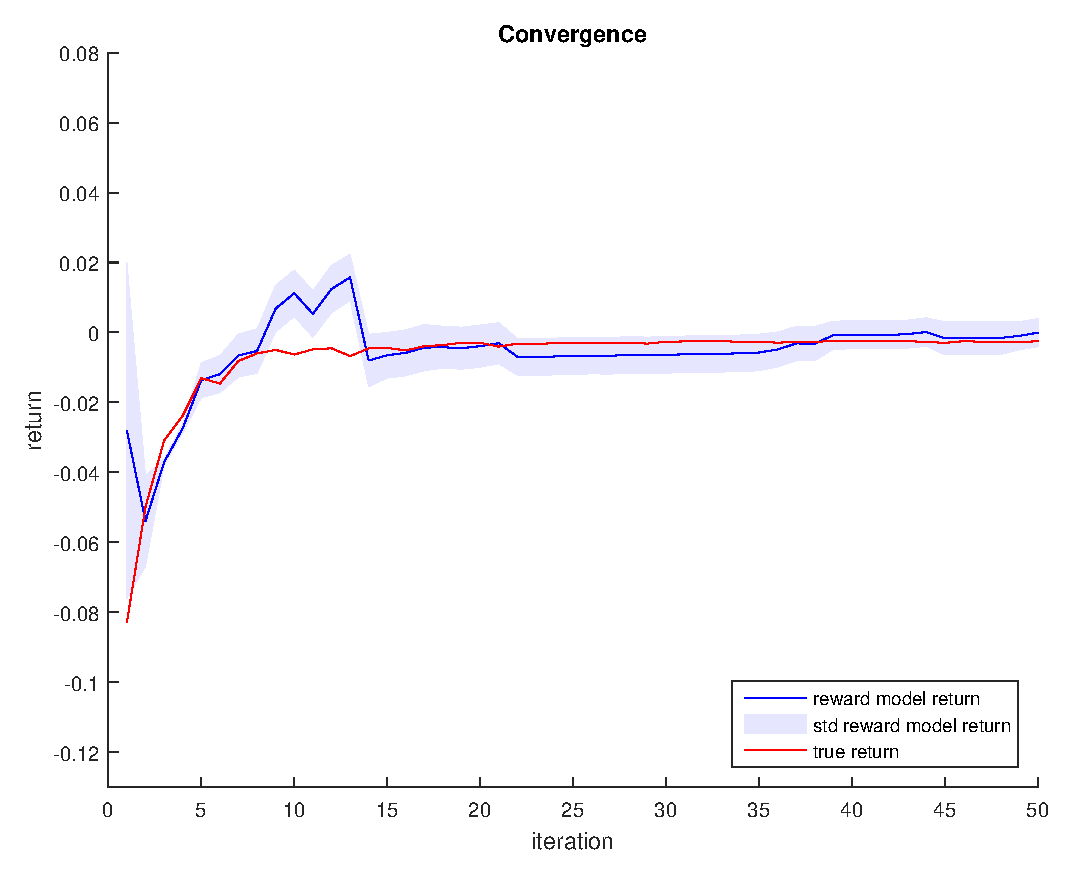
\includegraphics[width=\textwidth, keepaspectratio=1]{figures/results/advancedx/convergence_single_noise.eps}
        \caption{Convergence plot showing the return of the single GP reward model compared to the ``true'' return.}
        \label{fig:adx-single-noise-con}
    \end{minipage}%
    \begin{minipage}{0.5\textwidth}
        \centering
        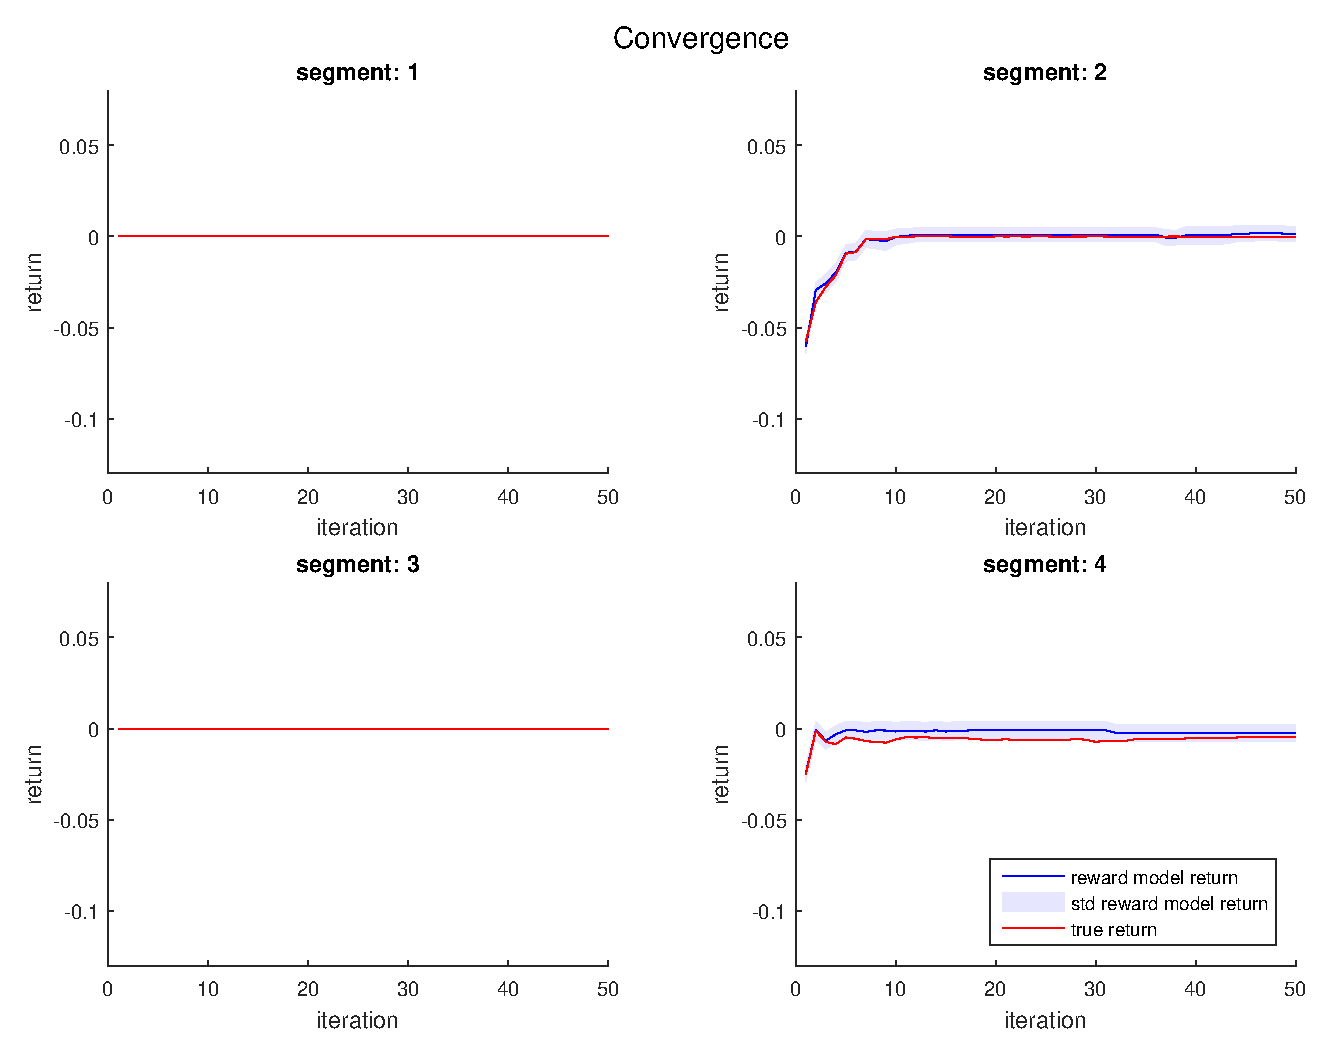
\includegraphics[width=\textwidth, keepaspectratio=1]{figures/results/advancedx/convergence_multi_noise.eps}
        \caption{Convergence plot showing the return of the multi GP reward model compared to the ``true'' return.}
        \label{fig:adx-multi-noise-con}
    \end{minipage}
\end{figure}

Since we still use only two feature functions for each segment, we can plot the reward function of the multi GP reward model. As can be seen in Figure \ref{fig:adx-multi-noise-reward} there are now two relevant time segments. The second time segment contains the viapoint and, as expected, there is an optimum clearly visible in the area of the viapoint. The second objective, is also clearly visible as an optimal line in two dimensional space.

% Reward function
\begin{figure}[!htb]
\centering
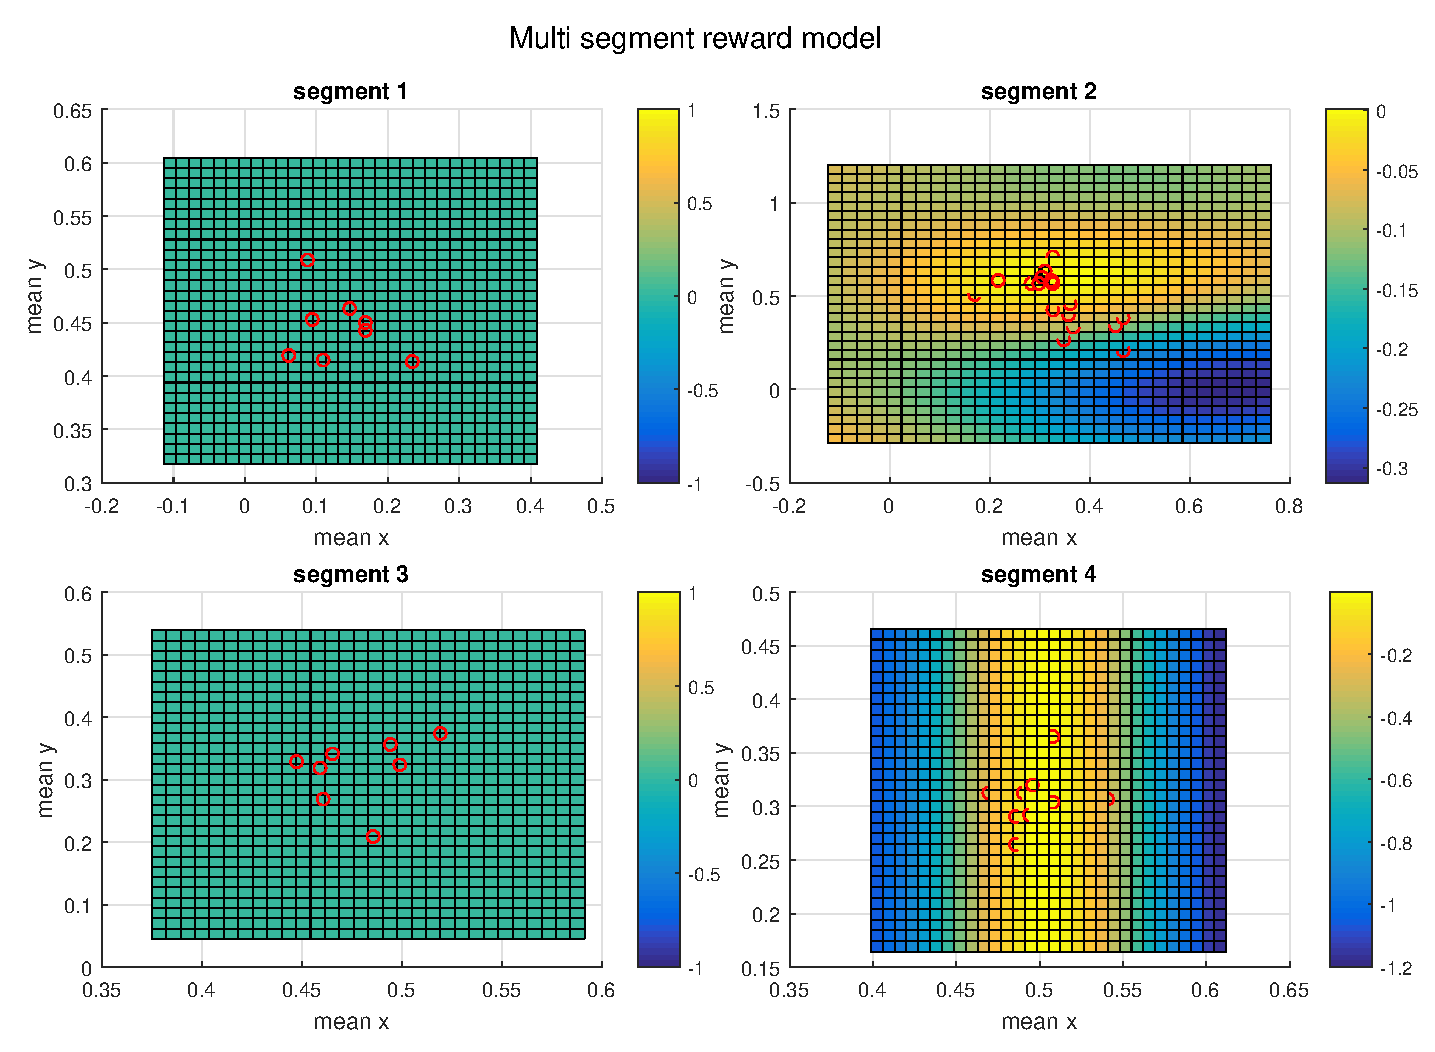
\includegraphics[width=\textwidth, keepaspectratio=1]{figures/results/advancedx/return_flat_multi_noise.eps}
\caption{Graphical representation of the resulting reward function of a multi GP reward model. The red dots represent queried rollouts. The black mark denotes the viapoint.}
\label{fig:adx-multi-noise-reward}
\end{figure}

If we look at the measurable results of the reward learning algorithms displayed in table \ref{tab:ad-com}, we can make some important remarks. First off,  it is clear that the multi GP reward model results in a policy that has better tracking results in both objectives compared to the single GP reward model. This suggests that a multi GP reward model is able to distinguish tasks in different time segments with more accuracy than a single GP reward model. If we look at the number of expert queries we see that the single GP method still requires less demonstrations compared to the multi GP method. However, it is clear that this difference is due to the number of demonstrations required during the initialization phase of the reward model. During learning, the multi GP reward model requires less expert ratings than the single GP reward model. 

If we compare the results of the reward learning methods with the results of the $\text{PI}^{BB}$ method, it is clear that a hard coded reward function still gives a better performance in terms of tracking. Especially if we look at the viapoint tracking results, we see an order of magnitude difference in performance.

\begin{table}[!htb]
    \centering
    \caption{Results of segmented active reward learning and $\text{PI}^{BB}$ applied to a viapoint/viaplane task using a computer expert.}
    \label{tab:ad-com}
    \begin{tabular}{|p{6cm}|c|c|c|c|}
        \hline
        Measure & single GP & multi GP &  $\text{PI}^{BB}$ & Unit \\ \hline \hline
        Average distance viapoint & $4.18 \cdot 10^{-2}$ & $2.00 \cdot 10^{-2}$ & $1.68 \cdot 10^{-2}$ & \si{m}  \\ \hline
        Standard deviation distance viapoint & $5.09 \cdot 10^{-2}$ & $1.14 \cdot 10^{-2}$ & $1.34 \cdot 10^{-2}$ & \si{m} \\ \hline
        Average SSE viaplane & $4.9 \cdot 10^{-3}$ & $8.3 \cdot 10^{-3}$ & $1.70 \cdot 10^{-4}$ & \si{m}  \\ \hline
        Standard deviation SSE viaplane & $5.7 \cdot 10^{-3}$ & $5.4 \cdot 10^{-3}$ & $1.9 \cdot 10^{-4}$ & \si{m} \\ \hline
        Initial number expert queries & 8 & 32 & 0 & - \\ \hline
        Average number expert queries & 45.05 & 52.2 & 0 & - \\ \hline
        Standard deviation number expert queries & 14.92 & 9.35 & 0 &  - \\ \hline
    \end{tabular}
\end{table}


\subsection{Manual expert result}
The performance of the multi objective task is comparable with that of the single viapoint task, as can be seen in Figure \ref{fig:adx-single-manual-traject} and Figure \ref{fig:adx-multi-manual-traject}. If we look at the accuracy concerning the viapoint we observe that the algorithm performs at least as good as the computer expert. It appears that we do not need to sacrifice a bit of performance in the first objective to achieve a good result for the second objective as is the case using a computer expert. Also, the single GP method performs shows a better trajectory then the multi GP method. This is in contrast to the results we saw earlier in Section \ref{sec:com-ad}. 

% Trajectory
\begin{figure}[!htb]
    \begin{minipage}[b]{\linewidth}
        \centering
        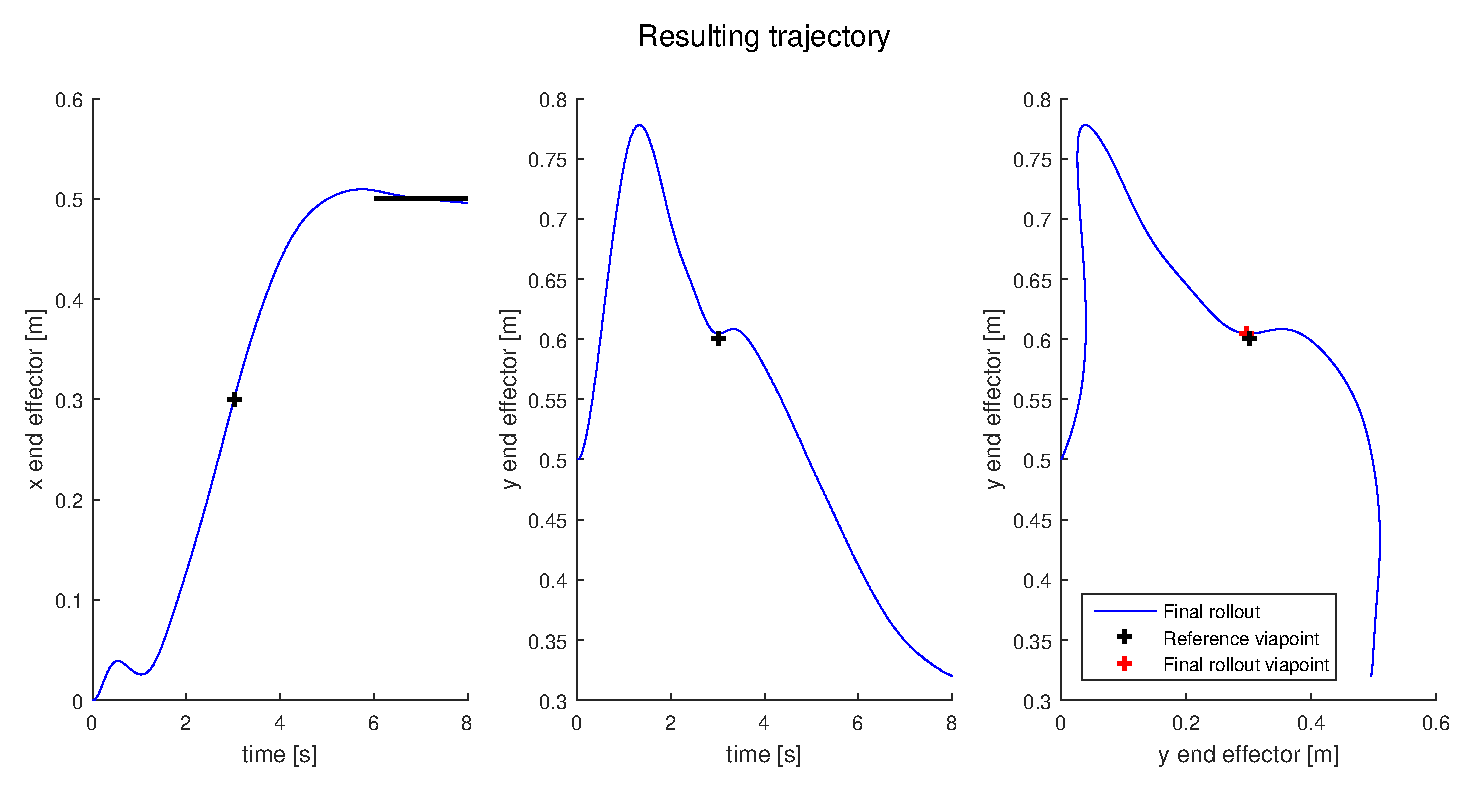
\includegraphics[width=\textwidth, height = 6 cm]{figures/results/advancedx/trajectory_single_manual.eps}
        \caption{Resulting trajectory of a multi objective task using a single GP reward model.}
        \label{fig:adx-single-manual-traject}
        \vspace{4ex}
    \end{minipage}%%
    
    \begin{minipage}[b]{\linewidth}
        \centering
        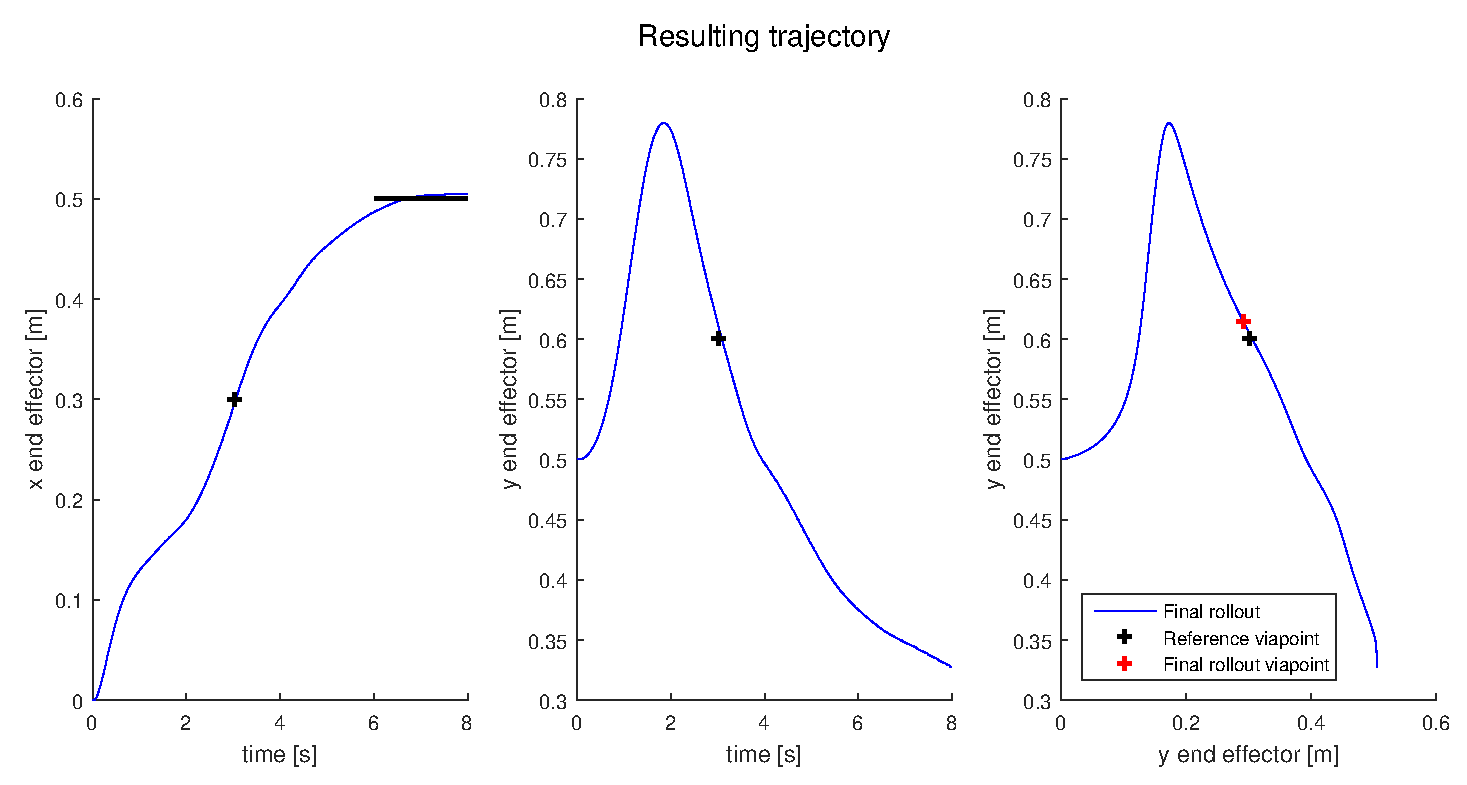
\includegraphics[width=\textwidth, height = 6 cm]{figures/results/advancedx/trajectory_multi_manual.eps}
        \caption{Resulting trajectory of a multi objective task using a multi GP reward model.}
        \label{fig:adx-multi-manual-traject}
    \end{minipage}%%
\end{figure}

The reward learning results are on display in Figure \ref{fig:adx-single-manual-con} and Figure \ref{fig:adx-multi-manual-con}. In Section \ref{sec:vp}, we showed the convergence results of the multi GP reward model in the same format as we did with the single GP reward model. Now that we have more than one relevant time segment we will present the results of the multi GP reward model per segment as is shown in Figure \ref{fig:adx-multi-manual-con}. We can make a few remarks regarding the convergence of the multi objective task. If we look at the multi GP reward model we can also conclude that the focus of the algorithm in terms of segments occurs in batches. In the first half of the learning phase, the algorithm only provides demonstrations in the last segment. Only when this objective seems to be learned, the focus shifts to the second segment in order to improve the viapoint objective. 

\begin{figure}[!htb]
    \centering
    \begin{minipage}{.5\textwidth}
        \centering
        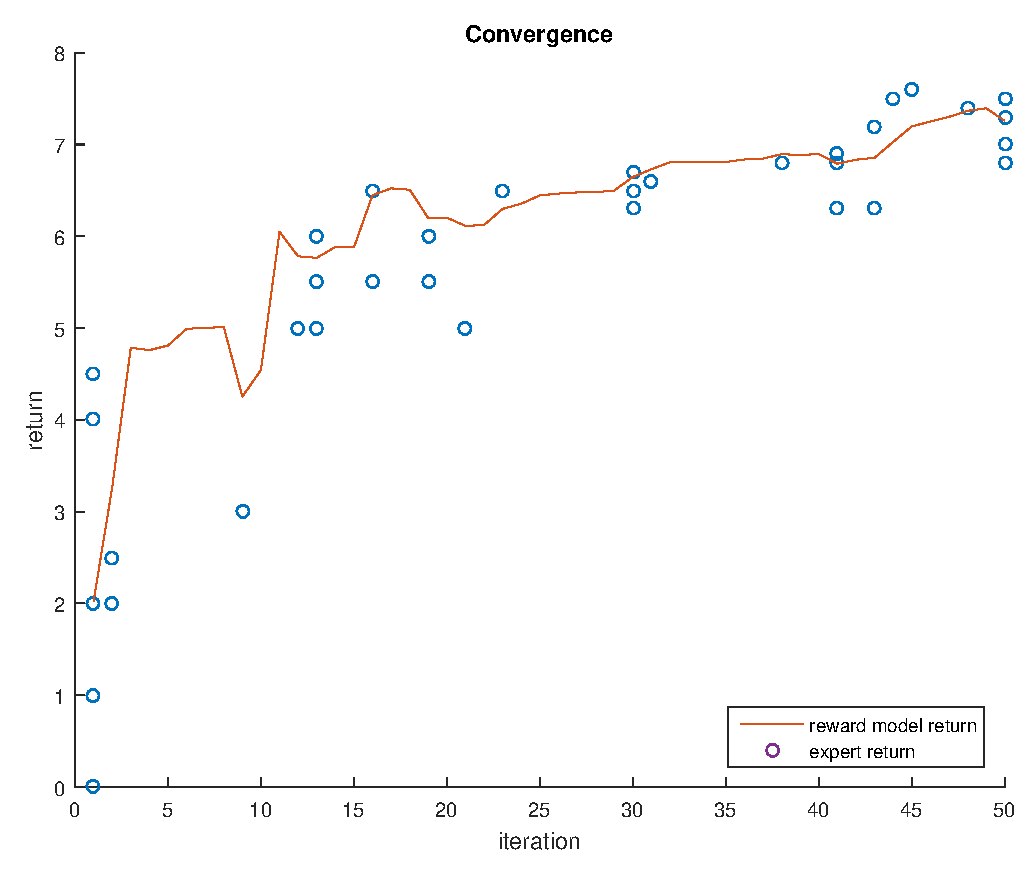
\includegraphics[width=\textwidth, keepaspectratio=1]{figures/results/advancedx/convergence_single_manual.eps}
        \caption{Convergence plot showing the return of the single GP reward model compared to the expert return.}
        \label{fig:adx-single-manual-con}
    \end{minipage}%
    \begin{minipage}{0.5\textwidth}
        \centering
        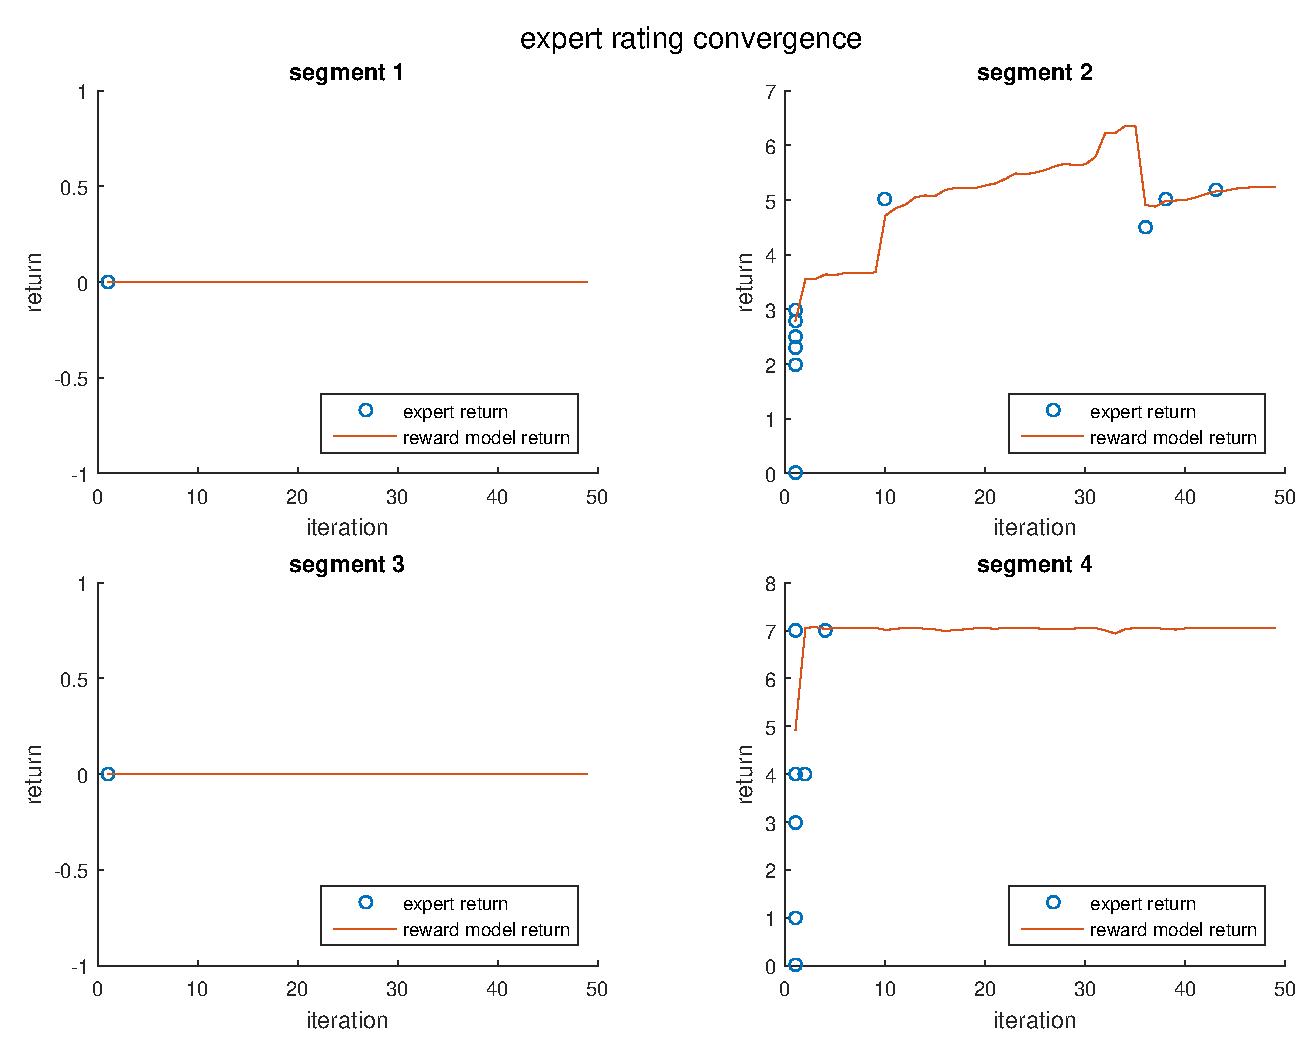
\includegraphics[width=\textwidth, keepaspectratio=1]{figures/results/advancedx/convergence_multi_manual.eps}
        \caption{Convergence plot showing the return of the multi GP reward model compared to the expert return.}
        \label{fig:adx-multi-manual-con}
    \end{minipage}
\end{figure}

If we look at the resulting reward function in Figure \ref{fig:adx-multi-manual-reward} we see something interesting. In the second segment we should observe a single optimal point right at the coordinate of the viapoint. Instead it is clear that the reward function does not care about the $x$ coordinate of the end effector. This can be explained when we look at the resulting trajectory. The $x$ coordinate of the first rollout is already close to the viapoints $x$ coordinate. Therefore, it is more important for the agent to learn the $y$ coordinate of the viapoint. If the reward function is constant in the $x$ direction, the agent will not learn significant changes in this dimension which is observed if we look at the demonstrated resulting trajectory.

% Reward function
\begin{figure}[!htb]
\centering
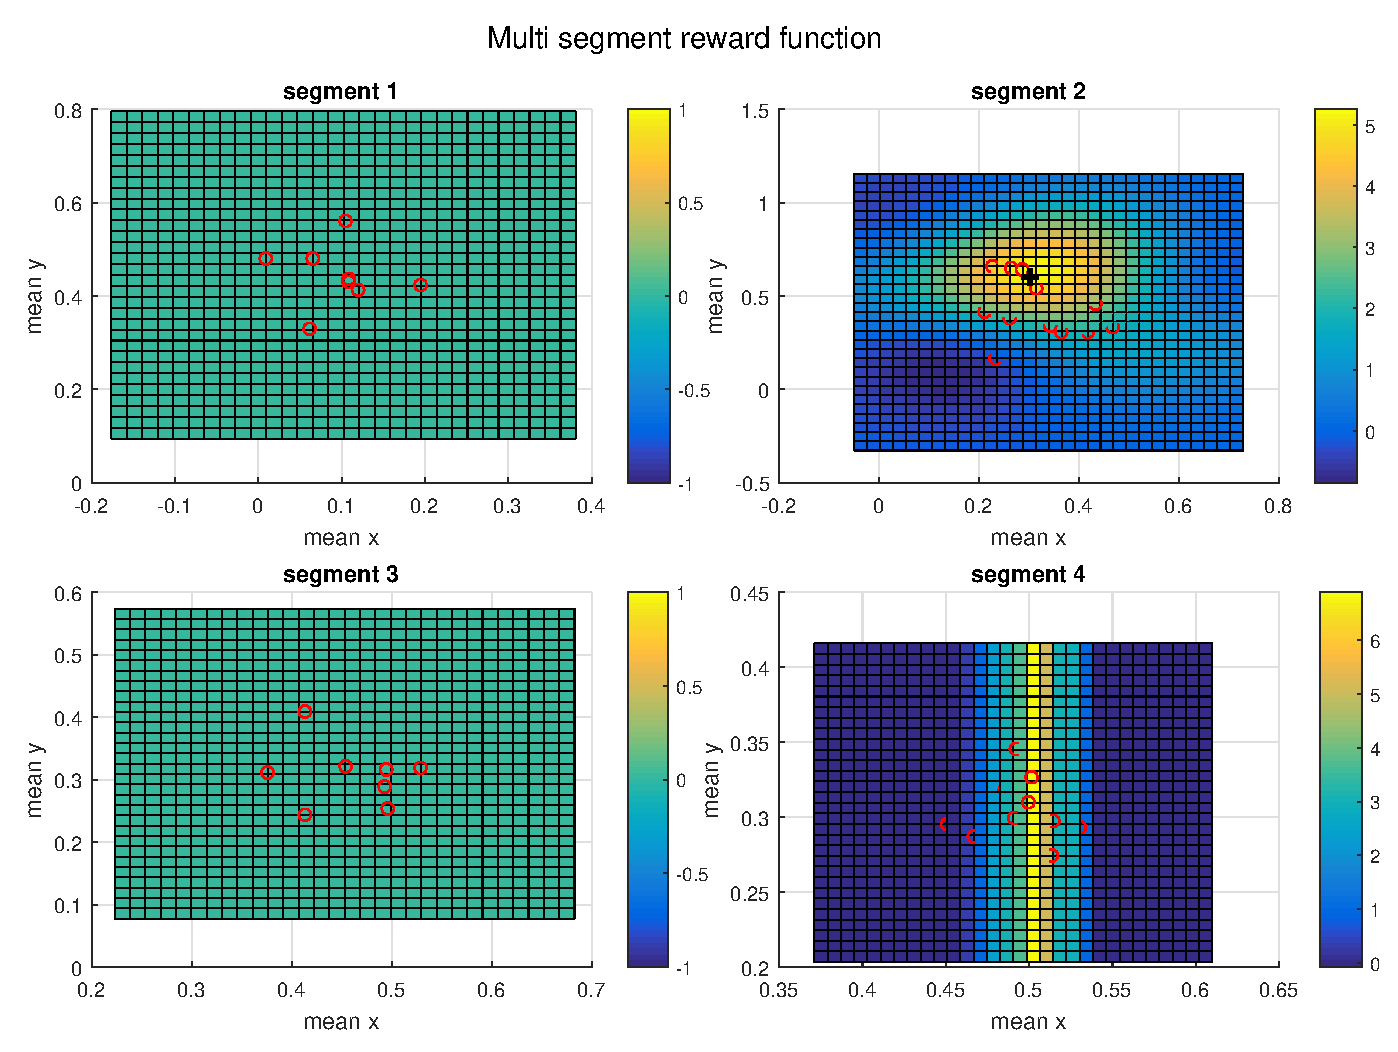
\includegraphics[width=\textwidth, keepaspectratio=1]{figures/results/advancedx/return_flat_multi_manual.eps}
\caption{Graphical representation of the resulting reward function of a multi GP reward model. The red dots represent queried rollouts. The black mark denotes the viapoint.}
\label{fig:adx-multi-manual-reward}
\end{figure}

A summary of the results of the new multi objective task using a human expert is shown in Table \ref{tab:ad-human}. We cannot objectively state which reward model is the better choice for this task since both methods are able to perform quite well. In terms of viapoint and viaplane tracking, the single GP reward model gives a better result over a multi GP reward model but in terms of expert queries we should chose a multi GP reward model. 

The two trials that are on display in the table are performing exceptionally well. This does not hold for all trials performed. There is an element of chance involved in teaching the robot a certain task, which is related to the acquisition function. In general, the acquisition function chooses which rollouts are interesting for demonstration. In the design of the acquisition function, we chose take the expected policy divergence as a measure of acquisition, which means that the acquisition function does not take into account the expected return. Poorly performing rollouts can be just as interesting as far as the acquisition function is concernded. However, it can happen that one of the demonstrated queries is tracking the viapoint of viaplane with a high accuracy. The expert can exploit this demonstration by giving such a demonstration a rating relatively higher then any other previous demonstration, hereby creating a ``spike'' in the reward model. This spike will cause the policy learner to converge to a very accurate result.

Extending the task description from a single viapoint to a multi objective task has implications for the human expert as well. When a single GP reward model is used, an obvious disadvantage is that the complexity for rating a rollout increases. The human expert has to keep track of the relative performance of different rollouts for two objectives and summarize this difference in one single grade. The most obvious advantage of using a multi GP reward model is the benefit in rating complexity. The expert only has to focus on one objective per demonstrated trajectory segment (provided that the objectives do not share a time segment). But there are disadvantages as well. In the previous section, the expert was free to choose what rating scale he or she liked. This does not hold for a multi objective task, due to the fact that the difference in priority between the two objectives is dependent on the reward. If one objective is scaled from one to hundred whilst the second objective is scaled from one to five, the reinforcement learning agent as well as the acquisition function will only focus on the former objective. During rating it is observed that the time segments which need most improvement according to the expert are not always the time segments that are queried. This problem is that the active reward learning algorithm assumes that the acquisition function provides useful demonstrations for the reward model. 

\begin{table}[!htb]
    \centering
    \caption{Results of segmented active reward learning and $\text{PI}^{BB}$ applied to a viapoint/viaplane task using a human expert.}
    \label{tab:ad-human}
    \begin{tabular}{|p{6cm}|c|c|c|c|}
        \hline
        Measure & single GP & multi GP & RL & Unit \\ \hline \hline
        Distance viapoint & $6.2 \cdot 10^{-3}$ & $ 1.7 \cdot 10^{-2}$ & $1.68 \cdot 10^{-2}$ & \si{m}  \\ \hline
        Squared error viaplane & $2.8 \cdot 10^{-3}$ & $5.6 \cdot 10^{-3}$ & $1.70 \cdot 10^{-4}$ & \si{m}  \\ \hline
        Initial number expert queries & 8 & 32 & 0 & - \\ \hline
        Number expert queries & 41 & 36 & 0 &  - \\ \hline
    \end{tabular}
\end{table}


\section{Multi objective task with tracking improvement}
\label{sec:ad-var}
In Section \ref{sec:ad} the results of a multi objective task are shown. Reviewing the results we can conclude the second objective, the viaplane tracking task, is prone for improvement. The reward model used in the previous section only uses the average position of the end effector as an input for the Gaussian process, and this information is not enough for the reinforcement learning agent to learn a viaplane task. 

In this section we will extend the reward model to include the variance of the end effector $x$ and $y$ position. This extension should give the reinforcement learning agent an incentive to keep the last segment of the trajectory as flat as possible. The cost for this extension is an increase in complexity for the reward model. Both the single GP and the multi GP reward model will have twice as much inputs as before.


\subsection{Computer expert result}
Besides an extension on the reward model, the rest of the algorithm does not have to be altered in order to work. For example the computer expert used in Section \ref{sec:ad} can be reused. If we look at the resulting trajectories (Figure \ref{fig:adxvar-single-noise-traject} and Figure \ref{fig:adxvar-single-noise-traject}) we can see an improvement in tracking performance. As can be seen in the plots, the standard deviation of the resulting trajectories around the viapoint and the viaplane is smaller compared to the results obtained in Section \ref{sec:ad}. It can also be concluded that the multi GP reward model has a smaller standard deviation around the objective and therefore has a better tracking performance.

% Single viapoint task


% Trajectory
\begin{figure}[!htb]
    \centering
    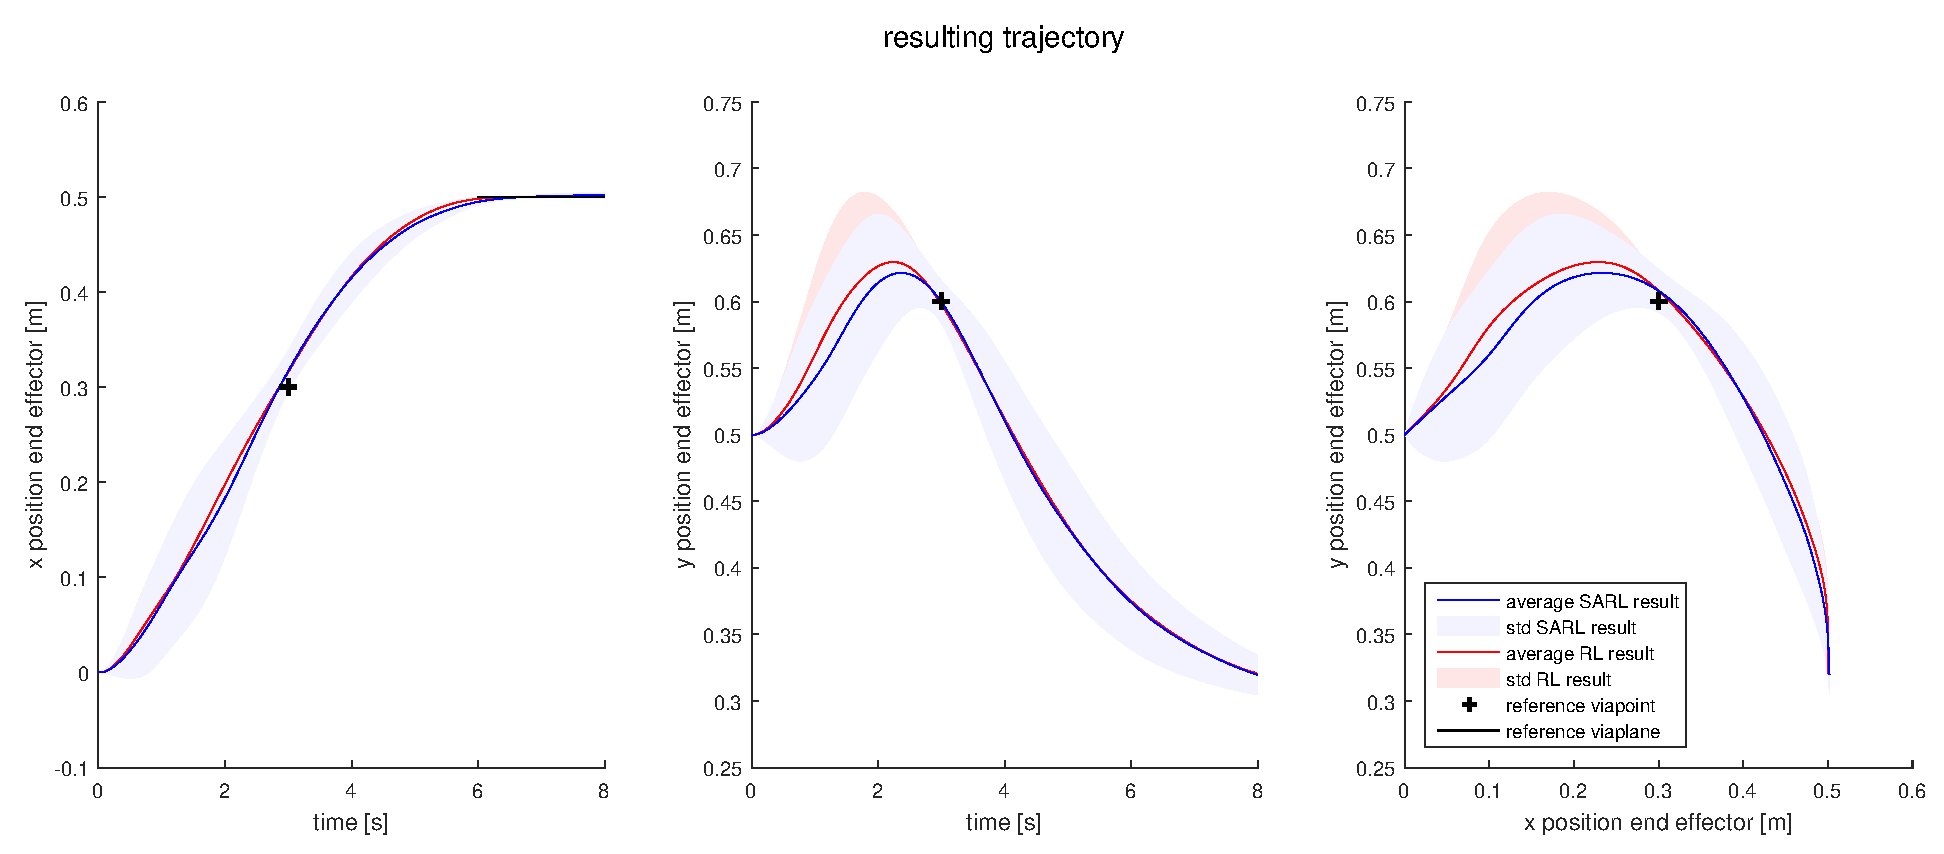
\includegraphics[width=\textwidth, height = 6 cm]{figures/results/advancedx-var/trajectory_single_noise_sum.eps}
    \caption{Resulting trajectories of a multi objective task using a single GP reward model.}
    \label{fig:adxvar-single-noise-traject}
\end{figure}
    
\begin{figure}
    \centering
    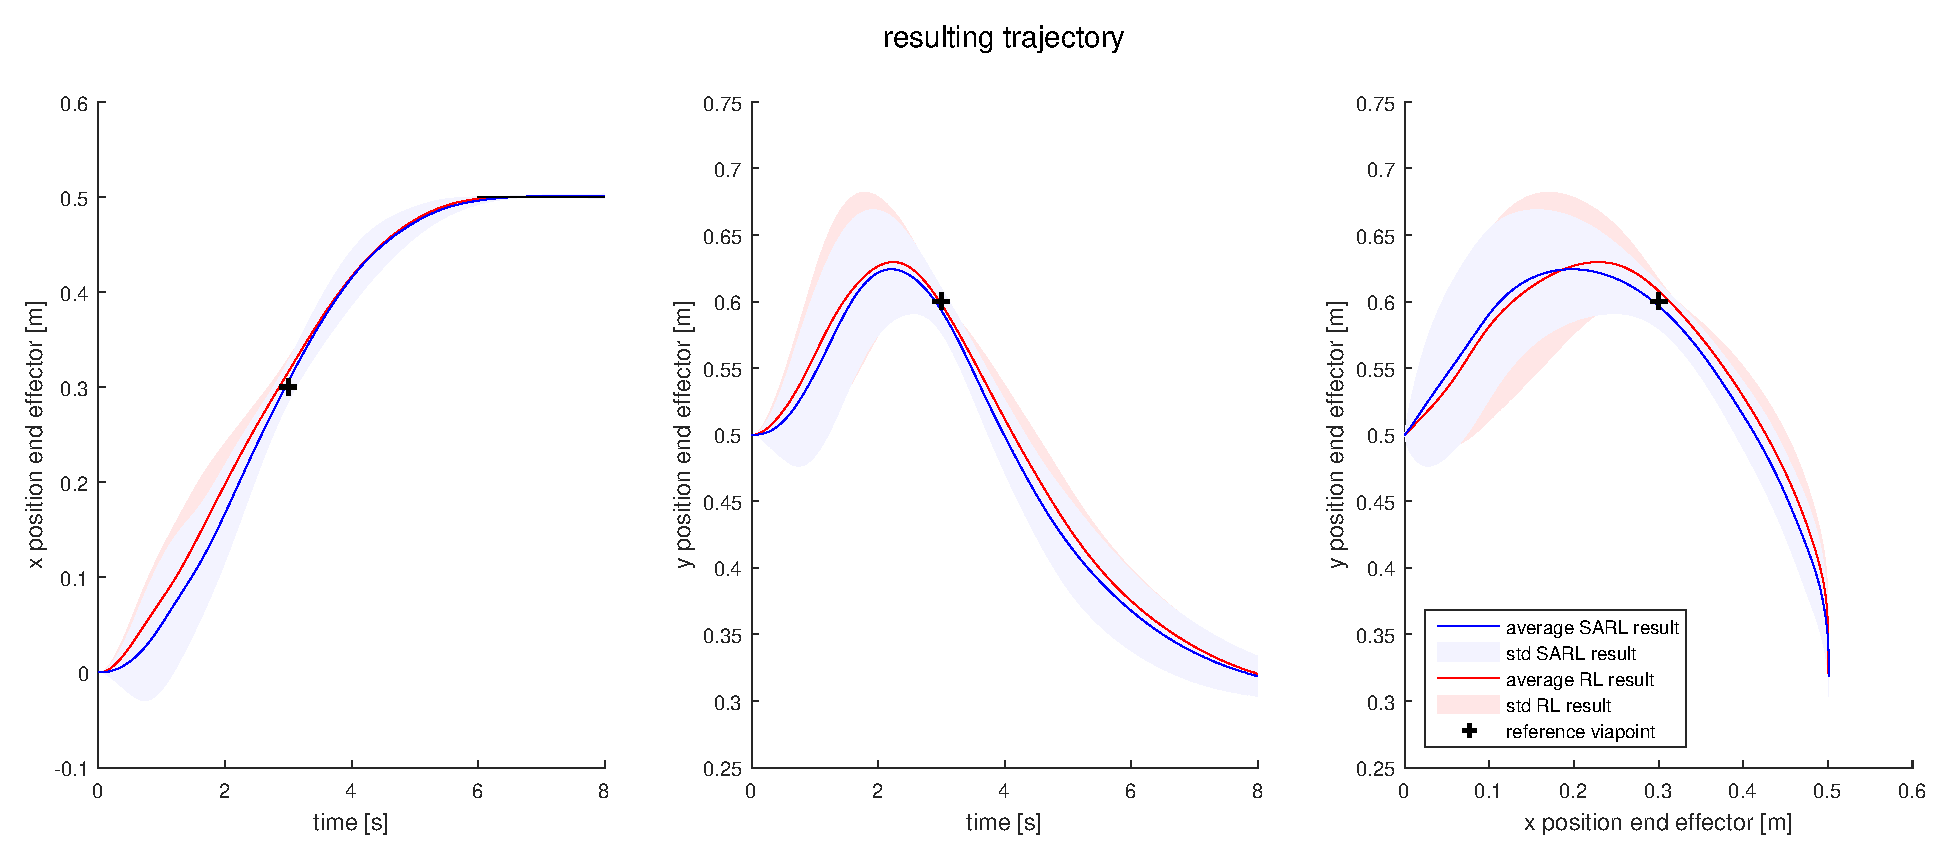
\includegraphics[width=\textwidth, height = 6 cm]{figures/results/advancedx-var/trajectory_multi_noise_sum.eps}
    \caption{Resulting trajectories of a multi objective task using a multi GP reward model.}
    \label{fig:adxvar-multi-noise-traject}
\end{figure}

The reward learning results, are also different depending on what reward model we use. It is clear in the convergence plots (Figure \ref{fig:adxvar-single-noise-con} and Figure \ref{fig:adxvar-multi-noise-con}) that the multi GP reward model is a much more accurate reward learner for this task. A reason for the decrease in reward learning for the single GP reward model can be found in the increased complexity of the Gaussian process. The GPs used for in the previous sections had a total number of eight inputs. The reward model used in this section has sixteen. An important aspect of reward learning is the ability for the reward model to determine which inputs are relevant for performance and which inputs can be safely ignored. Since we doubled the number of inputs for the single GP reward model, we increased the difficulty for the reward model to make this generalization as well. We also increased the number of inputs for the multi GP reward model but since we use a different GP for each segment, the number of inputs per GP stays relatively low. 

% results single gp. 

\begin{figure}[!htb]
    \centering
    \begin{minipage}{.5\textwidth}
        \centering
        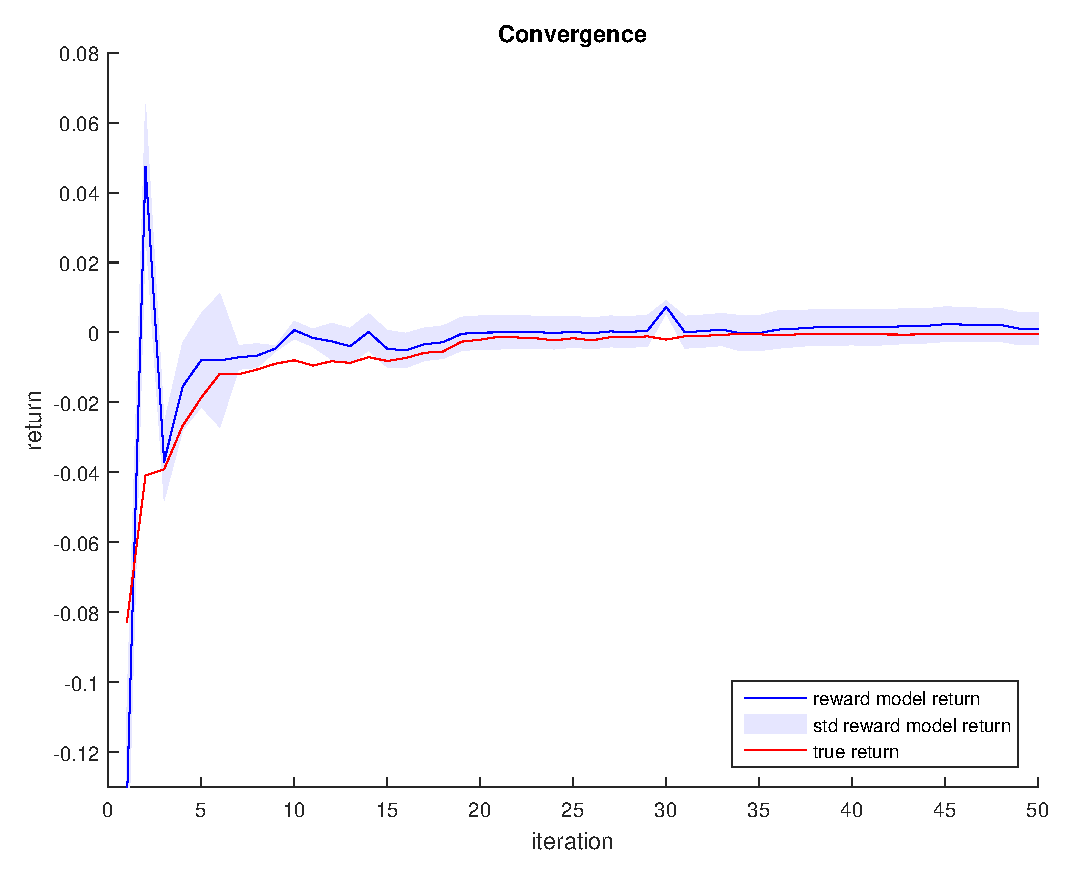
\includegraphics[width=\textwidth, keepaspectratio=1]{figures/results/advancedx-var/convergence_single_noise.eps}
        \caption{Convergence plot showing the return of the single GP reward model compared to the expert return.}
        \label{fig:adxvar-single-noise-con}
    \end{minipage}%
    \begin{minipage}{0.5\textwidth}
        \centering
        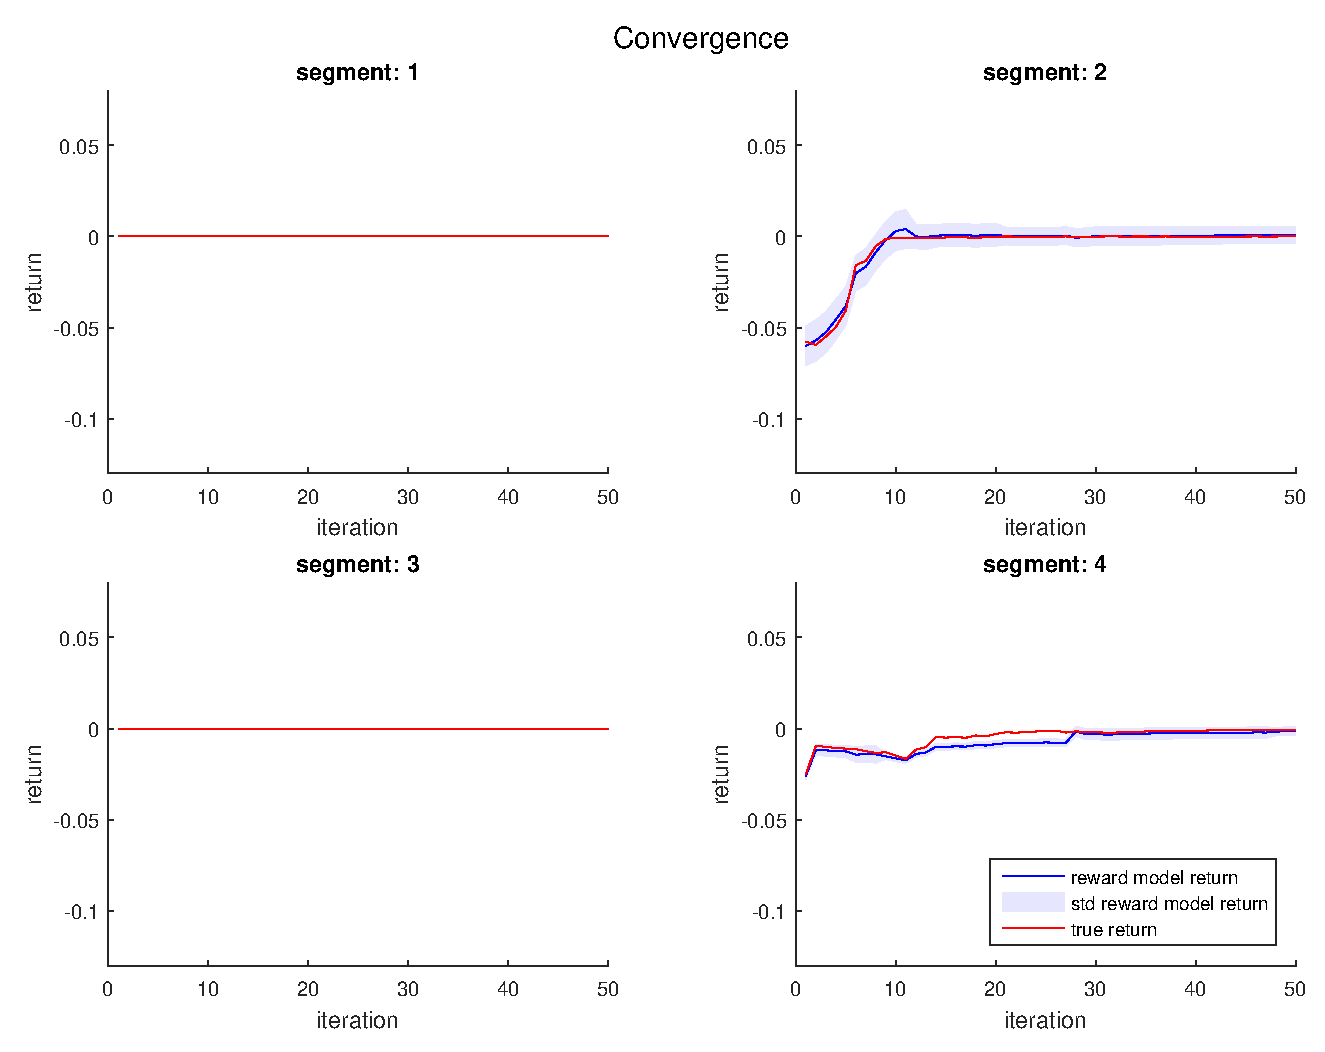
\includegraphics[width=\textwidth, keepaspectratio=1]{figures/results/advancedx-var/convergence_multi_noise.eps}
        \caption{Convergence plot showing the return of the multi GP reward model compared to the expert return.}
        \label{fig:adxvar-multi-noise-con}
    \end{minipage}
\end{figure}

% results multi gp

If we look at the measurable criteria in Table \ref{tab:ad-var-com}, it is clear that the variance extension of the reward model does have a positive effect on the results. First off, it can be noted that the SSE of the viaplane has dropped significantly compared to the results obtained in section \ref{sec:ad}. Another positive result is that the average distance to the viapoint also dropped, especially in case of the single GP method. The number of expert queries has increased slightly for both types of reward model. As before, the multi GP reward model needs some more expert queries than the single GP reward model, mostly due to the initialization phase of the algorithm.

\begin{table}[!htb]
    \centering
    \caption{Results of segmented active reward learning and $\text{PI}^{BB}$ applied to a viapoint/viaplane task using a computer expert.}
    \label{tab:ad-var-com}
    \begin{tabular}{|p{6cm}|c|c|c|c|}
        \hline
        Measure & single GP & multi GP & RL & Unit \\ \hline \hline
        Average distance viapoint & $2.79 \cdot 10^{-2}$ & $2.35 \cdot 10^{-2}$ & $1.68 \cdot 10^{-2}$ & \si{m}  \\ \hline
        Standard deviation distance viapoint & $1.35 \cdot 10^{-2}$ & $1.45 \cdot 10^{-2}$ & $1.34 \cdot 10^{-2}$ & \si{m} \\ \hline
        Average SSE viaplane & $1.7 \cdot 10^{-3}$ & $1.0 \cdot 10^{-3}$ & $1.70 \cdot 10^{-4}$ & \si{m}  \\ \hline
        Standard deviation SSE viaplane & $1.6 \cdot 10^{-3}$ & $1.5 \cdot 10^{-3}$ & $1.90 \cdot 10^{-4}$ & \si{m} \\ \hline
        Initial number expert queries & 8 & 32 & 0 & - \\ \hline
        Average number expert queries & 49.5 & 54.1 & 0 &  - \\ \hline
        Standard deviation number expert queries & 15.25 & 7.65 & 0 &  - \\ \hline 
    \end{tabular}
\end{table}

\clearpage

\subsection{Manual expert result}
In contrast the computer expert results, there is no performance increase when rating is done by a human expert. Although the reward models are able to take the variance of a trajectory segment into account, it is hard for the expert to do the rating. There is a clear increase rating complexity if the human expert does not only have reward staying close to a plane but also staying flat. Some rollouts for example have a very flat last trajectory segment, but on a different level than is aimed for. These rollouts should be rewarded as well for staying flat, but to the human expert this is counter intuitive.

In the resulting trajectories, shown in Figure \ref{fig:adxvar-single-manual-traject} and Figure \ref{fig:adxvar-multi-manual-traject}, it can clearly be observed that the extended reward model does not have a positive effect on the results. In the last segment of the trajectory, the end effector should track the viaplane nicely as was observed in the results of the computer expert. It is clear both reward models did not learn to reward the desired variance. 

If we examine the convergence plot, displayed in Figure \ref{fig:adxvar-single-manual-con} and Figure \ref{fig:adxvar-multi-manual-con}, it is also clear that the multi GP reward model does not give the second objective enough priority. As can be seen in the convergence plot of Figure \ref{fig:adxvar-multi-manual-con}, it is evident that the majority of demonstrations is performed in the second segment. This is probably one of the reasons why the multi GP reward model fails to include the variance input in its result. 

% Trajectory
\begin{figure}[!htb]
    \centering
    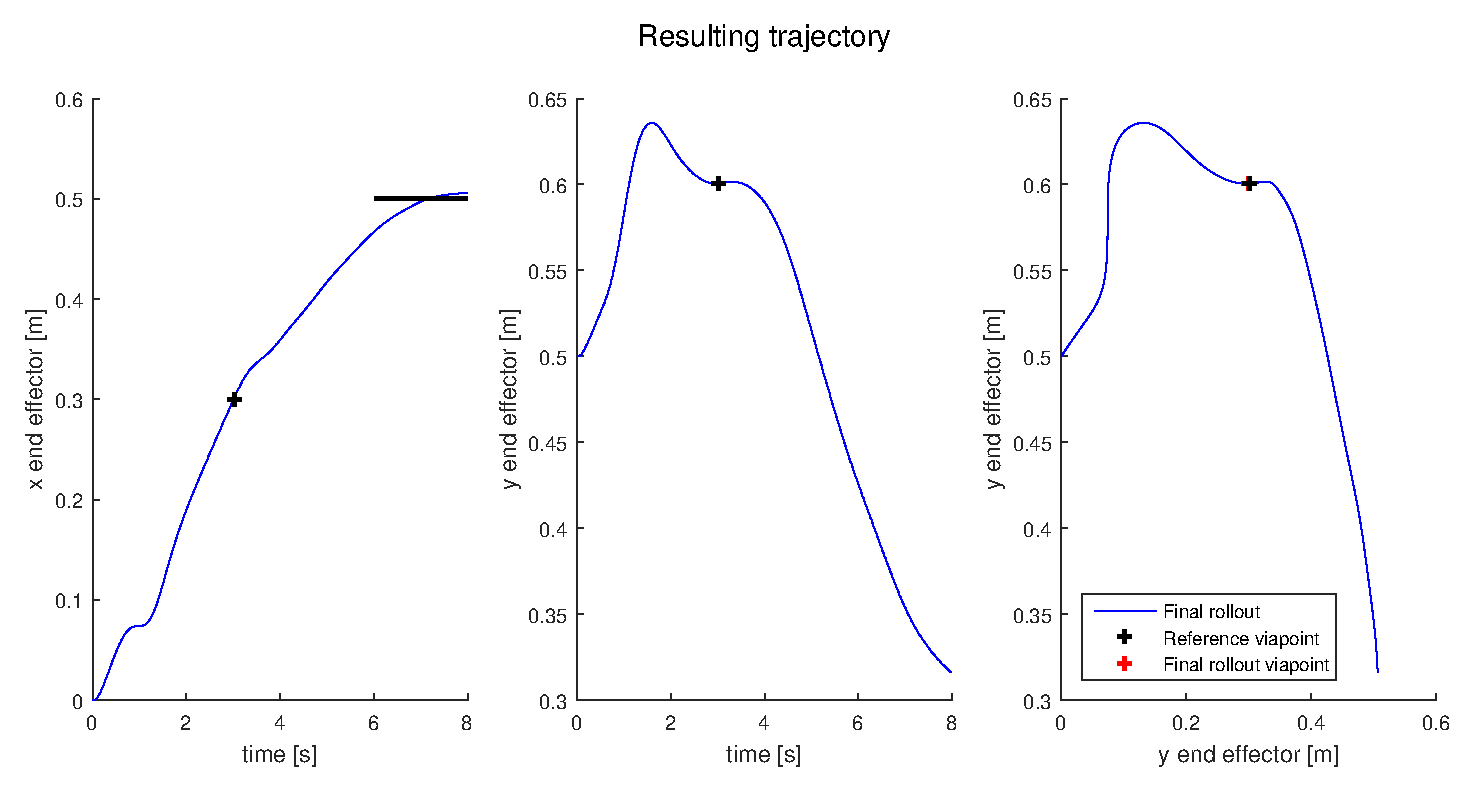
\includegraphics[width=\textwidth, height = 6 cm]{figures/results/advancedx-var/trajectory_single_manual.eps}
    \caption{Resulting trajectories of a multi objective point task using a single GP reward model.}
    \label{fig:adxvar-single-manual-traject}    
\end{figure}
   
\begin{figure}[!htb] 
    \centering
    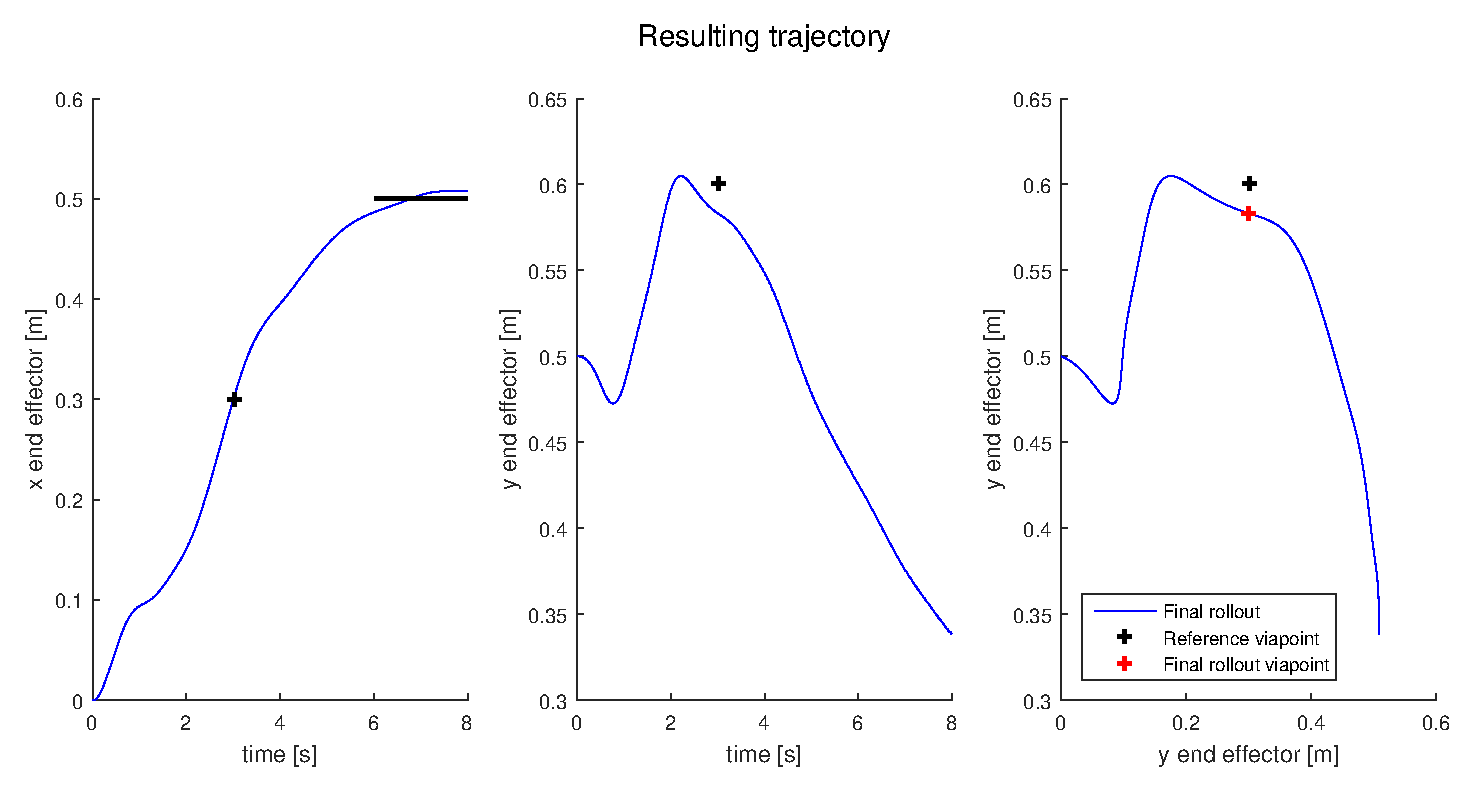
\includegraphics[width=\textwidth, height = 6 cm]{figures/results/advancedx-var/trajectory_multi_manual.eps}
    \caption{Resulting trajectories of a multi objective task using a multi GP reward model.}
    \label{fig:adxvar-multi-manual-traject}
\end{figure}

\begin{figure}[!htb]
    \centering
    \begin{minipage}{.5\textwidth}
        \centering
        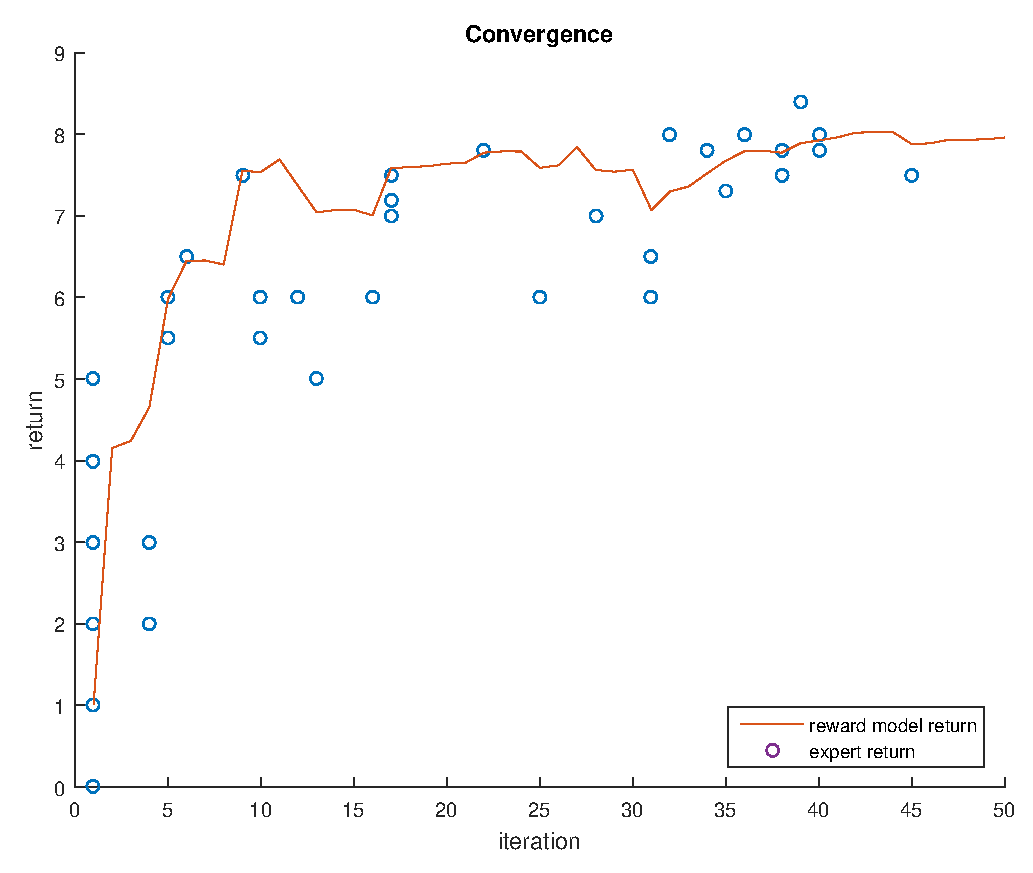
\includegraphics[width=\textwidth, keepaspectratio=1]{figures/results/advancedx-var/convergence_single_manual.eps}
        \caption{Convergence plot showing the return of the single GP reward model compared to the expert return.}
        \label{fig:adxvar-single-manual-con}
    \end{minipage}%
    \begin{minipage}{0.5\textwidth}
        \centering
        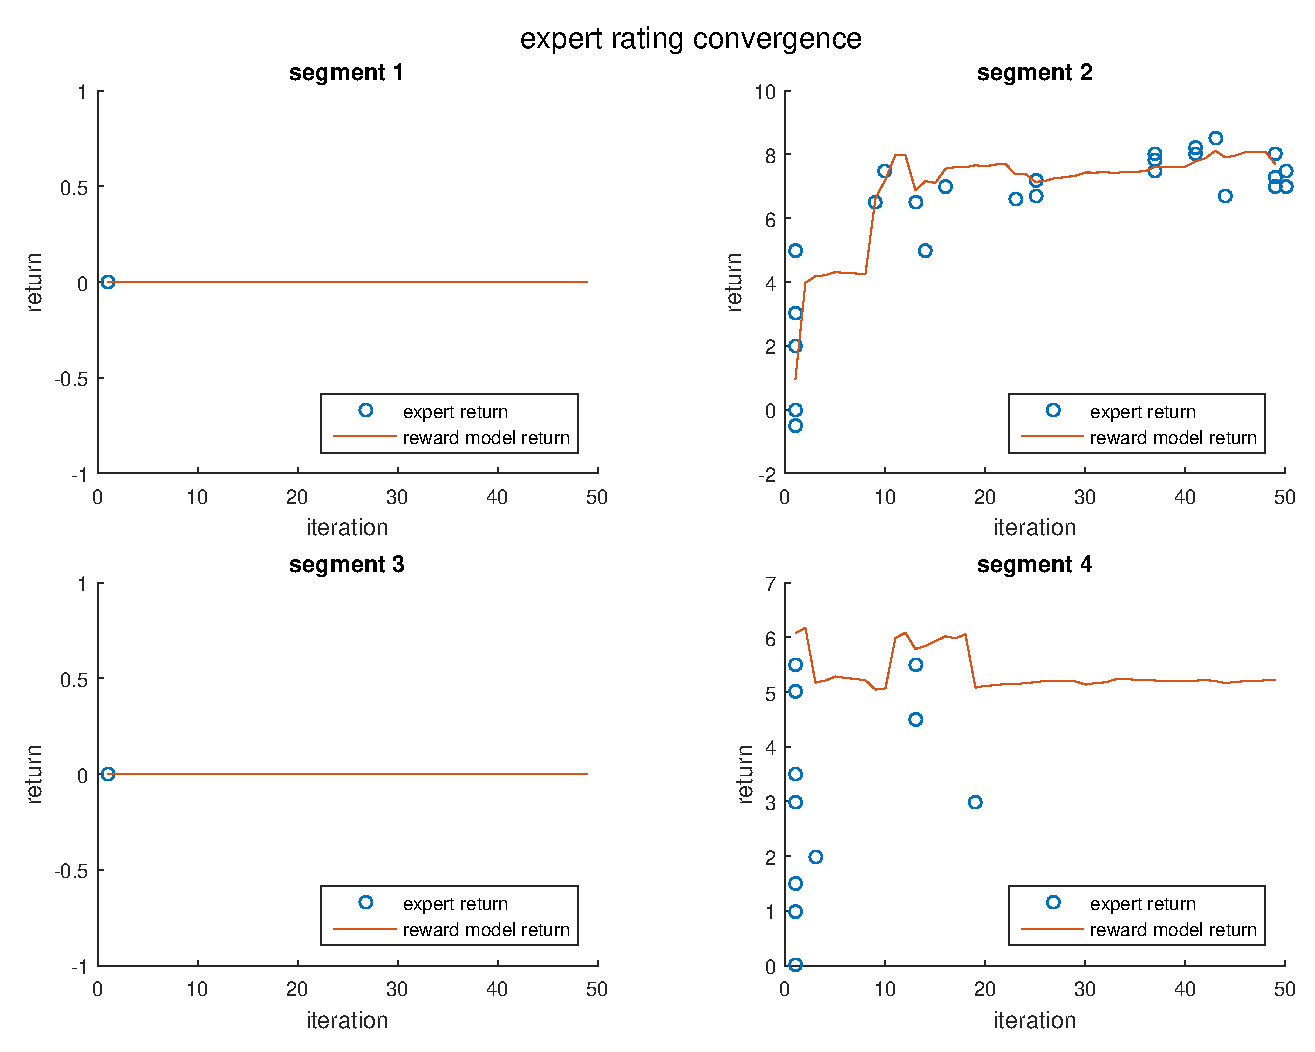
\includegraphics[width=\textwidth, keepaspectratio=1]{figures/results/advancedx-var/convergence_multi_manual.eps}
        \caption{Convergence plot showing the return of the multi GP reward model compared to the expert return.}
        \label{fig:adxvar-multi-manual-con}
    \end{minipage}
\end{figure}

If we look at the objective measures, we can see a decrease in performance. Both in terms of tracking performance and number of expert queries, the extended reward model does more harm than good. We can conclude that, in contrast to the computer expert results, the extended reward model does not tend to increase the result. The disadvantages of increasing the complexity for the expert outweigh the advantages gained in learning the reward model with more information.

\begin{table}[!htb]
    \centering
    \caption{Results of segmented active reward learning and $\text{PI}^{BB}$ applied to a viapoint/viaplane task using a human expert.}
    \label{tab:ad-var-hum}
    \begin{tabular}{|p{6cm}|c|c|c|c|}
        \hline
        Measure & single GP & multi GP & RL & Unit \\ \hline \hline
        Distance viapoint & $1.3 \cdot 10^{-3}$ & $1.67 \cdot 10^{-2}$ & $1.68 \cdot 10^{-2}$ & \si{m}  \\ \hline
        Squared error viaplane & $3.69 \cdot 10^{-2}$ & $1.00 \cdot 10^{-2}$ &  $1.70 \cdot 10^{-4}$ & \si{m}  \\ \hline
        Initial number expert queries & 8 & 32 & 0 & - \\ \hline
        Total number expert queries & 37 & 59 & 0 &  - \\ \hline
    \end{tabular}
\end{table}

% results multi gp

% Bibliography
% \bibliographystyle{ieeetr}
% \printbib{bibliography}

\end{document}